% Options for packages loaded elsewhere
\PassOptionsToPackage{unicode}{hyperref}
\PassOptionsToPackage{hyphens}{url}
%
\documentclass[
]{article}
\usepackage{amsmath,amssymb}
\usepackage{lmodern}
\usepackage{iftex}
\ifPDFTeX
  \usepackage[T1]{fontenc}
  \usepackage[utf8]{inputenc}
  \usepackage{textcomp} % provide euro and other symbols
\else % if luatex or xetex
  \usepackage{unicode-math}
  \defaultfontfeatures{Scale=MatchLowercase}
  \defaultfontfeatures[\rmfamily]{Ligatures=TeX,Scale=1}
\fi
% Use upquote if available, for straight quotes in verbatim environments
\IfFileExists{upquote.sty}{\usepackage{upquote}}{}
\IfFileExists{microtype.sty}{% use microtype if available
  \usepackage[]{microtype}
  \UseMicrotypeSet[protrusion]{basicmath} % disable protrusion for tt fonts
}{}
\makeatletter
\@ifundefined{KOMAClassName}{% if non-KOMA class
  \IfFileExists{parskip.sty}{%
    \usepackage{parskip}
  }{% else
    \setlength{\parindent}{0pt}
    \setlength{\parskip}{6pt plus 2pt minus 1pt}}
}{% if KOMA class
  \KOMAoptions{parskip=half}}
\makeatother
\usepackage{xcolor}
\IfFileExists{xurl.sty}{\usepackage{xurl}}{} % add URL line breaks if available
\IfFileExists{bookmark.sty}{\usepackage{bookmark}}{\usepackage{hyperref}}
\hypersetup{
  pdftitle={Clustering methods},
  pdfauthor={Denaldo Lapi, Francesco Aristei, Samy Chouity},
  hidelinks,
  pdfcreator={LaTeX via pandoc}}
\urlstyle{same} % disable monospaced font for URLs
\usepackage[margin=1in]{geometry}
\usepackage{color}
\usepackage{fancyvrb}
\newcommand{\VerbBar}{|}
\newcommand{\VERB}{\Verb[commandchars=\\\{\}]}
\DefineVerbatimEnvironment{Highlighting}{Verbatim}{commandchars=\\\{\}}
% Add ',fontsize=\small' for more characters per line
\usepackage{framed}
\definecolor{shadecolor}{RGB}{248,248,248}
\newenvironment{Shaded}{\begin{snugshade}}{\end{snugshade}}
\newcommand{\AlertTok}[1]{\textcolor[rgb]{0.94,0.16,0.16}{#1}}
\newcommand{\AnnotationTok}[1]{\textcolor[rgb]{0.56,0.35,0.01}{\textbf{\textit{#1}}}}
\newcommand{\AttributeTok}[1]{\textcolor[rgb]{0.77,0.63,0.00}{#1}}
\newcommand{\BaseNTok}[1]{\textcolor[rgb]{0.00,0.00,0.81}{#1}}
\newcommand{\BuiltInTok}[1]{#1}
\newcommand{\CharTok}[1]{\textcolor[rgb]{0.31,0.60,0.02}{#1}}
\newcommand{\CommentTok}[1]{\textcolor[rgb]{0.56,0.35,0.01}{\textit{#1}}}
\newcommand{\CommentVarTok}[1]{\textcolor[rgb]{0.56,0.35,0.01}{\textbf{\textit{#1}}}}
\newcommand{\ConstantTok}[1]{\textcolor[rgb]{0.00,0.00,0.00}{#1}}
\newcommand{\ControlFlowTok}[1]{\textcolor[rgb]{0.13,0.29,0.53}{\textbf{#1}}}
\newcommand{\DataTypeTok}[1]{\textcolor[rgb]{0.13,0.29,0.53}{#1}}
\newcommand{\DecValTok}[1]{\textcolor[rgb]{0.00,0.00,0.81}{#1}}
\newcommand{\DocumentationTok}[1]{\textcolor[rgb]{0.56,0.35,0.01}{\textbf{\textit{#1}}}}
\newcommand{\ErrorTok}[1]{\textcolor[rgb]{0.64,0.00,0.00}{\textbf{#1}}}
\newcommand{\ExtensionTok}[1]{#1}
\newcommand{\FloatTok}[1]{\textcolor[rgb]{0.00,0.00,0.81}{#1}}
\newcommand{\FunctionTok}[1]{\textcolor[rgb]{0.00,0.00,0.00}{#1}}
\newcommand{\ImportTok}[1]{#1}
\newcommand{\InformationTok}[1]{\textcolor[rgb]{0.56,0.35,0.01}{\textbf{\textit{#1}}}}
\newcommand{\KeywordTok}[1]{\textcolor[rgb]{0.13,0.29,0.53}{\textbf{#1}}}
\newcommand{\NormalTok}[1]{#1}
\newcommand{\OperatorTok}[1]{\textcolor[rgb]{0.81,0.36,0.00}{\textbf{#1}}}
\newcommand{\OtherTok}[1]{\textcolor[rgb]{0.56,0.35,0.01}{#1}}
\newcommand{\PreprocessorTok}[1]{\textcolor[rgb]{0.56,0.35,0.01}{\textit{#1}}}
\newcommand{\RegionMarkerTok}[1]{#1}
\newcommand{\SpecialCharTok}[1]{\textcolor[rgb]{0.00,0.00,0.00}{#1}}
\newcommand{\SpecialStringTok}[1]{\textcolor[rgb]{0.31,0.60,0.02}{#1}}
\newcommand{\StringTok}[1]{\textcolor[rgb]{0.31,0.60,0.02}{#1}}
\newcommand{\VariableTok}[1]{\textcolor[rgb]{0.00,0.00,0.00}{#1}}
\newcommand{\VerbatimStringTok}[1]{\textcolor[rgb]{0.31,0.60,0.02}{#1}}
\newcommand{\WarningTok}[1]{\textcolor[rgb]{0.56,0.35,0.01}{\textbf{\textit{#1}}}}
\usepackage{graphicx}
\makeatletter
\def\maxwidth{\ifdim\Gin@nat@width>\linewidth\linewidth\else\Gin@nat@width\fi}
\def\maxheight{\ifdim\Gin@nat@height>\textheight\textheight\else\Gin@nat@height\fi}
\makeatother
% Scale images if necessary, so that they will not overflow the page
% margins by default, and it is still possible to overwrite the defaults
% using explicit options in \includegraphics[width, height, ...]{}
\setkeys{Gin}{width=\maxwidth,height=\maxheight,keepaspectratio}
% Set default figure placement to htbp
\makeatletter
\def\fps@figure{htbp}
\makeatother
\setlength{\emergencystretch}{3em} % prevent overfull lines
\providecommand{\tightlist}{%
  \setlength{\itemsep}{0pt}\setlength{\parskip}{0pt}}
\setcounter{secnumdepth}{-\maxdimen} % remove section numbering
\usepackage{booktabs}
\usepackage{longtable}
\usepackage{array}
\usepackage{multirow}
\usepackage{wrapfig}
\usepackage{float}
\usepackage{colortbl}
\usepackage{pdflscape}
\usepackage{tabu}
\usepackage{threeparttable}
\usepackage{threeparttablex}
\usepackage[normalem]{ulem}
\usepackage{makecell}
\usepackage{xcolor}
\ifLuaTeX
  \usepackage{selnolig}  % disable illegal ligatures
\fi

\title{Clustering methods}
\usepackage{etoolbox}
\makeatletter
\providecommand{\subtitle}[1]{% add subtitle to \maketitle
  \apptocmd{\@title}{\par {\large #1 \par}}{}{}
}
\makeatother
\subtitle{Hierarchical, Partitioning, and Model-based Clustering}
\author{Denaldo Lapi, Francesco Aristei, Samy Chouity}
\date{05 June 2022}

\begin{document}
\maketitle

\renewcommand*\contentsname{Outline}
{
\setcounter{tocdepth}{2}
\tableofcontents
}
Delete all the possible objects of R that could have been left in
memory:

\begin{Shaded}
\begin{Highlighting}[]
\FunctionTok{rm}\NormalTok{(}\AttributeTok{list =} \FunctionTok{ls}\NormalTok{())}
\end{Highlighting}
\end{Shaded}

At first, let's load the libraries we'll need:

\begin{itemize}
\tightlist
\item
  \emph{dplyr} and \emph{ggplot2} will help us with data manipulation
  and graphs, respectively.
\item
  \emph{kableExtra} will help us to print beautiful tables.
\item
  \emph{gridExtra} for arranging the layout of the graphs.
\item
  \emph{stats} computes hierarchical cluster analysis on a set of
  dissimilarities and methods for analyzing it ( \emph{hclust}).
\item
  \emph{cluster} to apply the \emph{agnes} (agglomerative hierarchical
  clustering) and the \emph{diana} (divisive hierarchical clustering).
\item
  \emph{gplots} computes heatmaps for visualizing the distance matrix.
\item
  \emph{factoextra} for MVA methods and graph the clustering structures.
\item
  \emph{FactoMineR} computes hierarchical clustering on principal
  components.
\end{itemize}

\begin{Shaded}
\begin{Highlighting}[]
\FunctionTok{library}\NormalTok{(dplyr)}
\FunctionTok{library}\NormalTok{(ggplot2)}
\FunctionTok{library}\NormalTok{(kableExtra)}
\FunctionTok{library}\NormalTok{(gridExtra)}
\FunctionTok{library}\NormalTok{(stats)}
\FunctionTok{library}\NormalTok{(gplots)}
\FunctionTok{library}\NormalTok{(cluster)}
\FunctionTok{library}\NormalTok{(factoextra)}
\FunctionTok{library}\NormalTok{(FactoMineR)}
\end{Highlighting}
\end{Shaded}

\hypertarget{exploratory-data-analysis}{%
\subsection{Exploratory data analysis}\label{exploratory-data-analysis}}

The dataset we are going to analyze is about prostate cancer. It
consists of p=12 variables of mixed type (8 continuous and 4
categorical) measured on a group of n=50 prostate cancer patients. These
patients have either stage 3 or stage 4 prostate cancer.

Load the data from the R image `Prostate.RData'.

\begin{Shaded}
\begin{Highlighting}[]
\FunctionTok{load}\NormalTok{(}\StringTok{"Prostate.RData"}\NormalTok{)}
\end{Highlighting}
\end{Shaded}

Check dimension:

\begin{Shaded}
\begin{Highlighting}[]
\FunctionTok{dim}\NormalTok{(Prostate)}
\end{Highlighting}
\end{Shaded}

\begin{verbatim}
## [1] 50 12
\end{verbatim}

We have 50 rows and 12 columns

Check the structure:

\begin{Shaded}
\begin{Highlighting}[]
\FunctionTok{str}\NormalTok{(Prostate)}
\end{Highlighting}
\end{Shaded}

\begin{verbatim}
## tibble [50 x 12] (S3: tbl_df/tbl/data.frame)
##  $ age: num [1:50] 80 80 66 71 72 79 73 76 72 78 ...
##  $ wt : num [1:50] 105 95 116 98 101 79 80 99 88 107 ...
##  $ pf : Factor w/ 4 levels "0","1","2","3": 3 1 1 1 1 3 1 1 1 1 ...
##  $ hx : Factor w/ 2 levels "0","1": 2 2 1 1 1 1 2 2 1 1 ...
##  $ sbp: num [1:50] 14 16 12 19 14 15 13 15 14 14 ...
##  $ dbp: num [1:50] 7 10 8 10 10 7 8 9 7 9 ...
##  $ ekg: Factor w/ 7 levels "0","1","2","3",..: 6 5 1 1 3 2 5 5 5 1 ...
##  $ hg : num [1:50] 8.5 14.5 14.9 15.1 16.4 ...
##  $ sz : num [1:50] 6 7 18 10 1 16 61 9 7 42 ...
##  $ sg : num [1:50] 5 9 12 11 9 13 12 11 12 11 ...
##  $ ap : num [1:50] 160 0.9 58.1 0.6 0.8 ...
##  $ bm : Factor w/ 2 levels "0","1": 2 1 1 1 1 2 1 1 1 1 ...
\end{verbatim}

We can print a portion (a sample of 10) of the table using kable and the
pipe operator:

\begin{Shaded}
\begin{Highlighting}[]
\NormalTok{Prostate }\SpecialCharTok{\%\textgreater{}\%}
  \FunctionTok{sample\_n}\NormalTok{(., }\DecValTok{10}\NormalTok{, }\AttributeTok{replace=}\ConstantTok{FALSE}\NormalTok{) }\SpecialCharTok{\%\textgreater{}\%} 
  \FunctionTok{kbl}\NormalTok{(}\AttributeTok{caption =} \StringTok{"Phoneme data set (sample of 20)"}\NormalTok{) }\SpecialCharTok{\%\textgreater{}\%}
  \FunctionTok{kable\_classic}\NormalTok{(}\AttributeTok{full\_width =}\NormalTok{ F, }\AttributeTok{html\_font =} \StringTok{"Cambria"}\NormalTok{)}
\end{Highlighting}
\end{Shaded}

\begin{table}

\caption{\label{tab:unnamed-chunk-6}Phoneme data set (sample of 20)}
\centering
\begin{tabular}[t]{r|r|l|l|r|r|l|r|r|r|r|l}
\hline
age & wt & pf & hx & sbp & dbp & ekg & hg & sz & sg & ap & bm\\
\hline
79 & 79 & 2 & 0 & 15 & 7 & 1 & 13.29883 & 16 & 13 & 28.8984375 & 1\\
\hline
65 & 99 & 0 & 0 & 13 & 8 & 0 & 14.39844 & 10 & 9 & 0.5999756 & 0\\
\hline
75 & 88 & 0 & 1 & 14 & 6 & 0 & 13.39844 & 31 & 13 & 21.5976562 & 1\\
\hline
70 & 94 & 0 & 0 & 15 & 7 & 1 & 13.69922 & 24 & 7 & 0.7999268 & 0\\
\hline
76 & 103 & 0 & 1 & 13 & 7 & 5 & 12.50000 & 4 & 8 & 0.5000000 & 0\\
\hline
70 & 91 & 0 & 1 & 16 & 9 & 3 & 15.89844 & 7 & 9 & 1.0000000 & 0\\
\hline
54 & 89 & 0 & 0 & 15 & 6 & 2 & 14.79883 & 8 & 13 & 1.1999512 & 1\\
\hline
74 & 113 & 0 & 1 & 11 & 8 & 4 & 14.19922 & 41 & 13 & 2.2998047 & 0\\
\hline
73 & 106 & 0 & 1 & 16 & 9 & 0 & 14.69922 & 11 & 11 & 36.8984375 & 0\\
\hline
74 & 107 & 0 & 0 & 14 & 9 & 5 & 14.39844 & 6 & 9 & 0.2999878 & 0\\
\hline
\end{tabular}
\end{table}

Let's now visualize some basic statistics on each of the data frame's
columns with \emph{summary}:

\begin{Shaded}
\begin{Highlighting}[]
\NormalTok{Prostate }\SpecialCharTok{\%\textgreater{}\%} 
  \FunctionTok{summary}\NormalTok{(.) }\SpecialCharTok{\%\textgreater{}\%} 
  \FunctionTok{kbl}\NormalTok{(}\AttributeTok{caption =} \StringTok{"Basic statistics. Cancer data set"}\NormalTok{) }\SpecialCharTok{\%\textgreater{}\%}
  \FunctionTok{kable\_classic}\NormalTok{(}\AttributeTok{full\_width =}\NormalTok{ F, }\AttributeTok{html\_font =} \StringTok{"Cambria"}\NormalTok{)}
\end{Highlighting}
\end{Shaded}

\begin{table}

\caption{\label{tab:unnamed-chunk-7}Basic statistics. Cancer data set}
\centering
\begin{tabular}[t]{l|l|l|l|l|l|l|l|l|l|l|l|l}
\hline
  &      age &       wt & pf & hx &      sbp &      dbp & ekg &       hg &       sz &       sg &       ap & bm\\
\hline
 & Min.   :52.00 & Min.   : 79.00 & 0:45 & 0:29 & Min.   :10.00 & Min.   : 6.00 & 0:19 & Min.   : 8.50 & Min.   : 0.0 & Min.   : 5.00 & Min.   :  0.2000 & 0:40\\
\hline
 & 1st Qu.:71.00 & 1st Qu.: 93.25 & 1: 3 & 1:21 & 1st Qu.:13.00 & 1st Qu.: 7.00 & 1: 6 & 1st Qu.:12.27 & 1st Qu.: 7.0 & 1st Qu.: 9.00 & 1st Qu.:  0.5000 & 1:10\\
\hline
 & Median :74.00 & Median : 99.00 & 2: 2 & NA & Median :14.00 & Median : 8.00 & 2: 3 & Median :13.50 & Median :12.5 & Median :11.00 & Median :  0.7999 & NA\\
\hline
 & Mean   :72.76 & Mean   : 98.44 & 3: 0 & NA & Mean   :14.38 & Mean   : 7.98 & 3: 3 & Mean   :13.35 & Mean   :15.9 & Mean   :10.12 & Mean   : 27.1210 & NA\\
\hline
 & 3rd Qu.:77.00 & 3rd Qu.:104.75 & NA & NA & 3rd Qu.:16.00 & 3rd Qu.: 9.00 & 4:13 & 3rd Qu.:14.70 & 3rd Qu.:20.0 & 3rd Qu.:11.75 & 3rd Qu.: 18.6230 & NA\\
\hline
 & Max.   :84.00 & Max.   :119.00 & NA & NA & Max.   :19.00 & Max.   :11.00 & 5: 6 & Max.   :18.20 & Max.   :61.0 & Max.   :14.00 & Max.   :596.0000 & NA\\
\hline
 & NA & NA & NA & NA & NA & NA & 6: 0 & NA & NA & NA & NA & NA\\
\hline
\end{tabular}
\end{table}

Since clustering methods we analyzed work by considering a continuous
domain, i.e.~continuous varaibles, we'll remove the cageorical ones.
Another possibility could be to encode them in some numeric way, but we
should take care of the distance measure to use in the hierarchial and
k-means algorithms, which is difficutl to express in case of categorical
variables.

Let's select only the numerical columns:

\begin{Shaded}
\begin{Highlighting}[]
\FunctionTok{library}\NormalTok{(purrr)}
\NormalTok{Prostate\_reduced }\OtherTok{=}\NormalTok{ Prostate[, }\FunctionTok{c}\NormalTok{(}\DecValTok{1}\NormalTok{,}\DecValTok{2}\NormalTok{,}\DecValTok{5}\NormalTok{,}\DecValTok{6}\NormalTok{,}\DecValTok{8}\NormalTok{,}\DecValTok{9}\NormalTok{,}\DecValTok{10}\NormalTok{,}\DecValTok{11}\NormalTok{)]}
\end{Highlighting}
\end{Shaded}

Let's now check again the structure:

\begin{Shaded}
\begin{Highlighting}[]
\FunctionTok{str}\NormalTok{(Prostate\_reduced)}
\end{Highlighting}
\end{Shaded}

\begin{verbatim}
## tibble [50 x 8] (S3: tbl_df/tbl/data.frame)
##  $ age: num [1:50] 80 80 66 71 72 79 73 76 72 78 ...
##  $ wt : num [1:50] 105 95 116 98 101 79 80 99 88 107 ...
##  $ sbp: num [1:50] 14 16 12 19 14 15 13 15 14 14 ...
##  $ dbp: num [1:50] 7 10 8 10 10 7 8 9 7 9 ...
##  $ hg : num [1:50] 8.5 14.5 14.9 15.1 16.4 ...
##  $ sz : num [1:50] 6 7 18 10 1 16 61 9 7 42 ...
##  $ sg : num [1:50] 5 9 12 11 9 13 12 11 12 11 ...
##  $ ap : num [1:50] 160 0.9 58.1 0.6 0.8 ...
\end{verbatim}

And the dimensions:

\begin{Shaded}
\begin{Highlighting}[]
\FunctionTok{dim}\NormalTok{(Prostate\_reduced)}
\end{Highlighting}
\end{Shaded}

\begin{verbatim}
## [1] 50  8
\end{verbatim}

\hypertarget{check-for-missing-values}{%
\subsubsection{Check for missing
values}\label{check-for-missing-values}}

Let's check for NA values:

\begin{Shaded}
\begin{Highlighting}[]
\FunctionTok{colSums}\NormalTok{((}\FunctionTok{is.na}\NormalTok{((Prostate\_reduced))))}
\end{Highlighting}
\end{Shaded}

\begin{verbatim}
## age  wt sbp dbp  hg  sz  sg  ap 
##   0   0   0   0   0   0   0   0
\end{verbatim}

There are no missing values!

\hypertarget{outliers}{%
\subsubsection{Outliers}\label{outliers}}

One way to check for multivariate outliers is to use the
\href{https://en.wikipedia.org/wiki/Mahalanobis_distance}{Malhanobis'
distance} . It can be thought of as a metric for estimating how far each
observation is from the center of all the variables' distributions
(i.e.~the centroid in the multivariate space).

We'll use the \emph{chemometrics} package, which contains a function
(`Moutlier') for calculating and plotting both the ``Mahalanobis'''
distance and a robust version of the ``Mahalanobis''' distance.

At first, let's calculate the ``Mahalanobis''' distances using the
`Moutlier' function, to which we provide as parameters the numeric data
frame, the quantile cutoff point beyond which we want to identify points
as outliers, and whether or not we want a plot:

\begin{Shaded}
\begin{Highlighting}[]
\CommentTok{\#install.packages("chemometrics")}
\FunctionTok{library}\NormalTok{(chemometrics)}
\end{Highlighting}
\end{Shaded}

\begin{verbatim}
## Warning: package 'chemometrics' was built under R version 4.1.3
\end{verbatim}

\begin{verbatim}
## Loading required package: rpart
\end{verbatim}

\begin{Shaded}
\begin{Highlighting}[]
\NormalTok{md }\OtherTok{\textless{}{-}} \FunctionTok{Moutlier}\NormalTok{(Prostate\_reduced, }\AttributeTok{quantile =} \FloatTok{0.975}\NormalTok{, }\AttributeTok{plot=}\ConstantTok{FALSE}\NormalTok{)}
\end{Highlighting}
\end{Shaded}

The function returns the cutoff value for the outliers:

\begin{Shaded}
\begin{Highlighting}[]
\NormalTok{md}\SpecialCharTok{$}\NormalTok{cutoff}
\end{Highlighting}
\end{Shaded}

\begin{verbatim}
## [1] 4.187427
\end{verbatim}

We simply use the `which' function to identify which cases are outliers
according to the `cutoff' value and in this way we obtain the outliers'
indexes:

\begin{Shaded}
\begin{Highlighting}[]
\NormalTok{outliers }\OtherTok{\textless{}{-}} \FunctionTok{which}\NormalTok{(md}\SpecialCharTok{$}\NormalTok{md }\SpecialCharTok{\textgreater{}}\NormalTok{ md}\SpecialCharTok{$}\NormalTok{cutoff)}
\FunctionTok{head}\NormalTok{(outliers, }\DecValTok{10}\NormalTok{) }\CommentTok{\# show first 10 outliers according to Malhanobis distance}
\end{Highlighting}
\end{Shaded}

\begin{verbatim}
## [1]  7 13
\end{verbatim}

One way for identifying multivariate outliers (non-parametric approach)
is to use the LOF (``local outlier factor'') algorithm, which identifies
density-based local outliers.

The algorithm we are going to use (from the package
\href{https://rdrr.io/cran/DDoutlier/man/LOF.html}{DDoutlier}) computes
a local density for observations with a given k-nearest neighbors (we
choose k = 5). This local density is compared to the density of the
respective nearest neighbors, resulting in the local outlier factor.

Therefore, the function returns a vector of LOF scores for each
observation: the greater the LOF, the greater the outlierness of the
data point.

\begin{Shaded}
\begin{Highlighting}[]
\CommentTok{\#install.packages(\textquotesingle{}DDoutlier\textquotesingle{})}
\FunctionTok{library}\NormalTok{(}\StringTok{"DDoutlier"}\NormalTok{)}
\end{Highlighting}
\end{Shaded}

\begin{verbatim}
## Warning: package 'DDoutlier' was built under R version 4.1.3
\end{verbatim}

\begin{Shaded}
\begin{Highlighting}[]
\NormalTok{lof }\OtherTok{\textless{}{-}} \FunctionTok{LOF}\NormalTok{(Prostate\_reduced, }\AttributeTok{k =} \DecValTok{5}\NormalTok{) }\CommentTok{\# outlier score with a neighborhood of 5 points}
\end{Highlighting}
\end{Shaded}

We can show the lof scores for the 5 first observations:

\begin{Shaded}
\begin{Highlighting}[]
\FunctionTok{head}\NormalTok{(lof)}
\end{Highlighting}
\end{Shaded}

\begin{verbatim}
## [1] 2.937176 1.076620 1.119548 1.087195 1.027537 1.254277
\end{verbatim}

We can see and visualize the distribution of outlier scores:

\begin{Shaded}
\begin{Highlighting}[]
\FunctionTok{summary}\NormalTok{(lof) }\CommentTok{\# some statistics}
\end{Highlighting}
\end{Shaded}

\begin{verbatim}
##    Min. 1st Qu.  Median    Mean 3rd Qu.    Max. 
##   0.921   1.035   1.111   1.460   1.376  10.829
\end{verbatim}

\begin{Shaded}
\begin{Highlighting}[]
\FunctionTok{hist}\NormalTok{(lof)}
\end{Highlighting}
\end{Shaded}

\includegraphics{clustering_files/figure-latex/unnamed-chunk-17-1.pdf}

It could be useful to plot also the sorted LOF scores:

\begin{Shaded}
\begin{Highlighting}[]
\FunctionTok{plot}\NormalTok{(}\FunctionTok{sort}\NormalTok{(lof), }\AttributeTok{type =} \StringTok{"l"}\NormalTok{,  }\AttributeTok{main =} \StringTok{"LOF (K = 5)"}\NormalTok{,}
  \AttributeTok{xlab =} \StringTok{"Points sorted by LOF"}\NormalTok{, }\AttributeTok{ylab =} \StringTok{"LOF"}\NormalTok{)}
\end{Highlighting}
\end{Shaded}

\includegraphics{clustering_files/figure-latex/unnamed-chunk-18-1.pdf}

Looks like outliers start around a LOF value of 2.0.

Let's show the indexes for 5 most outlying observations

\begin{Shaded}
\begin{Highlighting}[]
\NormalTok{lof\_with\_names }\OtherTok{=}\NormalTok{ lof}
\FunctionTok{names}\NormalTok{(lof\_with\_names) }\OtherTok{\textless{}{-}} \DecValTok{1}\SpecialCharTok{:}\FunctionTok{nrow}\NormalTok{(Prostate)}
\FunctionTok{sort}\NormalTok{(lof\_with\_names, }\AttributeTok{decreasing =} \ConstantTok{TRUE}\NormalTok{)[}\DecValTok{1}\SpecialCharTok{:}\DecValTok{5}\NormalTok{]}
\end{Highlighting}
\end{Shaded}

\begin{verbatim}
##        13         1        47        32        22 
## 10.829292  2.937176  2.788041  2.025857  1.946327
\end{verbatim}

Let's first find the indexes of the outliers with a lof score above 2.0:

\begin{Shaded}
\begin{Highlighting}[]
\NormalTok{outliers }\OtherTok{\textless{}{-}} \FunctionTok{which}\NormalTok{(lof }\SpecialCharTok{\textgreater{}} \FloatTok{2.0}\NormalTok{)}
\end{Highlighting}
\end{Shaded}

Number of detected outliers:

\begin{Shaded}
\begin{Highlighting}[]
\FunctionTok{length}\NormalTok{(outliers)}
\end{Highlighting}
\end{Shaded}

\begin{verbatim}
## [1] 4
\end{verbatim}

\begin{Shaded}
\begin{Highlighting}[]
\NormalTok{outliers}
\end{Highlighting}
\end{Shaded}

\begin{verbatim}
## [1]  1 13 32 47
\end{verbatim}

We will simply remove the found outliers (found with LOF) from the
dataset, considering that we have more than 4k observations:

\begin{Shaded}
\begin{Highlighting}[]
\NormalTok{Prostate\_no\_outliers }\OtherTok{=}\NormalTok{ Prostate\_reduced[}\SpecialCharTok{{-}}\NormalTok{outliers,] }
\end{Highlighting}
\end{Shaded}

Let's now check again the dimensions:

\begin{Shaded}
\begin{Highlighting}[]
\FunctionTok{dim}\NormalTok{(Prostate\_no\_outliers)}
\end{Highlighting}
\end{Shaded}

\begin{verbatim}
## [1] 46  8
\end{verbatim}

The outliers have been correctly removed!

\hypertarget{check-variables-distribution}{%
\subsubsection{Check variables
distribution}\label{check-variables-distribution}}

Check variables correlation:

\begin{Shaded}
\begin{Highlighting}[]
\FunctionTok{library}\NormalTok{(GGally)}
\end{Highlighting}
\end{Shaded}

\begin{verbatim}
## Registered S3 method overwritten by 'GGally':
##   method from   
##   +.gg   ggplot2
\end{verbatim}

\begin{Shaded}
\begin{Highlighting}[]
\FunctionTok{ggpairs}\NormalTok{(Prostate\_no\_outliers,}
        \AttributeTok{title=}\StringTok{"Correlation matrix. Phoneme data"}\NormalTok{)}
\end{Highlighting}
\end{Shaded}

\includegraphics{clustering_files/figure-latex/unnamed-chunk-25-1.pdf}

Let's now check the univariate distribution of each variable.

We'll use the density plot:

\begin{Shaded}
\begin{Highlighting}[]
\FunctionTok{library}\NormalTok{(gridExtra)}
\FunctionTok{library}\NormalTok{(ggplot2)}
\NormalTok{g1 }\OtherTok{\textless{}{-}} \FunctionTok{ggplot}\NormalTok{(Prostate\_no\_outliers, }\FunctionTok{aes}\NormalTok{(}\AttributeTok{x=}\NormalTok{age)) }\SpecialCharTok{+} \FunctionTok{geom\_density}\NormalTok{(}\AttributeTok{alpha=}\FloatTok{0.8}\NormalTok{)}
\NormalTok{g2 }\OtherTok{\textless{}{-}} \FunctionTok{ggplot}\NormalTok{(Prostate\_no\_outliers, }\FunctionTok{aes}\NormalTok{(}\AttributeTok{x=}\NormalTok{wt)) }\SpecialCharTok{+} \FunctionTok{geom\_density}\NormalTok{(}\AttributeTok{alpha=}\FloatTok{0.8}\NormalTok{)}
\NormalTok{g3 }\OtherTok{\textless{}{-}} \FunctionTok{ggplot}\NormalTok{(Prostate\_no\_outliers, }\FunctionTok{aes}\NormalTok{(}\AttributeTok{x=}\NormalTok{sbp)) }\SpecialCharTok{+} \FunctionTok{geom\_density}\NormalTok{(}\AttributeTok{alpha=}\FloatTok{0.8}\NormalTok{)}
\NormalTok{g4 }\OtherTok{\textless{}{-}} \FunctionTok{ggplot}\NormalTok{(Prostate\_no\_outliers, }\FunctionTok{aes}\NormalTok{(}\AttributeTok{x=}\NormalTok{dbp)) }\SpecialCharTok{+} \FunctionTok{geom\_density}\NormalTok{(}\AttributeTok{alpha=}\FloatTok{0.8}\NormalTok{)}
\NormalTok{g5 }\OtherTok{\textless{}{-}} \FunctionTok{ggplot}\NormalTok{(Prostate\_no\_outliers, }\FunctionTok{aes}\NormalTok{(}\AttributeTok{x=}\NormalTok{hg)) }\SpecialCharTok{+} \FunctionTok{geom\_density}\NormalTok{(}\AttributeTok{alpha=}\FloatTok{0.8}\NormalTok{)}
\NormalTok{g6 }\OtherTok{\textless{}{-}} \FunctionTok{ggplot}\NormalTok{(Prostate\_no\_outliers, }\FunctionTok{aes}\NormalTok{(}\AttributeTok{x=}\NormalTok{sz)) }\SpecialCharTok{+} \FunctionTok{geom\_density}\NormalTok{(}\AttributeTok{alpha=}\FloatTok{0.8}\NormalTok{)}
\NormalTok{g7 }\OtherTok{\textless{}{-}} \FunctionTok{ggplot}\NormalTok{(Prostate\_no\_outliers, }\FunctionTok{aes}\NormalTok{(}\AttributeTok{x=}\NormalTok{sg)) }\SpecialCharTok{+} \FunctionTok{geom\_density}\NormalTok{(}\AttributeTok{alpha=}\FloatTok{0.8}\NormalTok{)}
\NormalTok{g8 }\OtherTok{\textless{}{-}} \FunctionTok{ggplot}\NormalTok{(Prostate\_no\_outliers, }\FunctionTok{aes}\NormalTok{(}\AttributeTok{x=}\NormalTok{ap)) }\SpecialCharTok{+} \FunctionTok{geom\_density}\NormalTok{(}\AttributeTok{alpha=}\FloatTok{0.8}\NormalTok{)}

\FunctionTok{grid.arrange}\NormalTok{(g1,g2, }\AttributeTok{nrow=}\DecValTok{1}\NormalTok{); }\FunctionTok{grid.arrange}\NormalTok{(g3,g4,}\AttributeTok{nrow=}\DecValTok{1}\NormalTok{);}\FunctionTok{grid.arrange}\NormalTok{(g5,g6,}\AttributeTok{nrow=}\DecValTok{1}\NormalTok{); }\FunctionTok{grid.arrange}\NormalTok{(g7,g8,}\AttributeTok{nrow=}\DecValTok{1}\NormalTok{)}
\end{Highlighting}
\end{Shaded}

\includegraphics{clustering_files/figure-latex/unnamed-chunk-26-1.pdf}
\includegraphics{clustering_files/figure-latex/unnamed-chunk-26-2.pdf}
\includegraphics{clustering_files/figure-latex/unnamed-chunk-26-3.pdf}
\includegraphics{clustering_files/figure-latex/unnamed-chunk-26-4.pdf}

A better approach for a visual inspection is the \emph{Q-Q plot}, which
shows the distribution of the data against the expected normal
distribution. In particular, for normally distributed data, observations
should lie approximately on a straight line. If the data is non-normal,
the points form a curve that deviates markedly from a straight line.
Let's perform such plot for each predictor, by using the library
\emph{ggpubr}:

\begin{Shaded}
\begin{Highlighting}[]
\FunctionTok{library}\NormalTok{(gridExtra)}
\FunctionTok{library}\NormalTok{(ggpubr)}
\FunctionTok{library}\NormalTok{(ggplot2)}

\NormalTok{g1 }\OtherTok{\textless{}{-}} \FunctionTok{ggqqplot}\NormalTok{(Prostate\_no\_outliers, }\AttributeTok{x=}\StringTok{"age"}\NormalTok{, }\AttributeTok{col=}\DecValTok{2}\NormalTok{, }\AttributeTok{ggtheme =} \FunctionTok{theme\_gray}\NormalTok{(), }\AttributeTok{title =} \StringTok{"age Q{-}Q plot"}\NormalTok{)}
\NormalTok{g2 }\OtherTok{\textless{}{-}} \FunctionTok{ggqqplot}\NormalTok{(Prostate\_no\_outliers, }\AttributeTok{x=}\StringTok{"wt"}\NormalTok{, }\AttributeTok{col=}\DecValTok{2}\NormalTok{, }\AttributeTok{ggtheme =} \FunctionTok{theme\_gray}\NormalTok{(), }\AttributeTok{title =} \StringTok{"wt Q{-}Q plot"}\NormalTok{)}
\NormalTok{g3 }\OtherTok{\textless{}{-}} \FunctionTok{ggqqplot}\NormalTok{(Prostate\_no\_outliers, }\AttributeTok{x=}\StringTok{"sbp"}\NormalTok{, }\AttributeTok{col=}\DecValTok{2}\NormalTok{, }\AttributeTok{ggtheme =} \FunctionTok{theme\_gray}\NormalTok{(), }\AttributeTok{title =} \StringTok{"sbp Q{-}Q plot"}\NormalTok{)}
\NormalTok{g4 }\OtherTok{\textless{}{-}} \FunctionTok{ggqqplot}\NormalTok{(Prostate\_no\_outliers, }\AttributeTok{x=}\StringTok{"dbp"}\NormalTok{, }\AttributeTok{col=}\DecValTok{2}\NormalTok{, }\AttributeTok{ggtheme =} \FunctionTok{theme\_gray}\NormalTok{(), }\AttributeTok{title =} \StringTok{"dbp Q{-}Q plot"}\NormalTok{)}
\NormalTok{g5 }\OtherTok{\textless{}{-}} \FunctionTok{ggqqplot}\NormalTok{(Prostate\_no\_outliers, }\AttributeTok{x=}\StringTok{"hg"}\NormalTok{, }\AttributeTok{col=}\DecValTok{2}\NormalTok{, }\AttributeTok{ggtheme =} \FunctionTok{theme\_gray}\NormalTok{(), }\AttributeTok{title =} \StringTok{"hg Q{-}Q plot"}\NormalTok{)}
\NormalTok{g6 }\OtherTok{\textless{}{-}} \FunctionTok{ggqqplot}\NormalTok{(Prostate\_no\_outliers, }\AttributeTok{x=}\StringTok{"sz"}\NormalTok{, }\AttributeTok{col=}\DecValTok{2}\NormalTok{, }\AttributeTok{ggtheme =} \FunctionTok{theme\_gray}\NormalTok{(), }\AttributeTok{title =} \StringTok{"sz Q{-}Q plot"}\NormalTok{)}
\NormalTok{g7 }\OtherTok{\textless{}{-}} \FunctionTok{ggqqplot}\NormalTok{(Prostate\_no\_outliers, }\AttributeTok{x=}\StringTok{"sg"}\NormalTok{, }\AttributeTok{col=}\DecValTok{2}\NormalTok{, }\AttributeTok{ggtheme =} \FunctionTok{theme\_gray}\NormalTok{(), }\AttributeTok{title =} \StringTok{"sg Q{-}Q plot"}\NormalTok{)}
\NormalTok{g8 }\OtherTok{\textless{}{-}} \FunctionTok{ggqqplot}\NormalTok{(Prostate\_no\_outliers, }\AttributeTok{x=}\StringTok{"ap"}\NormalTok{, }\AttributeTok{col=}\DecValTok{2}\NormalTok{, }\AttributeTok{ggtheme =} \FunctionTok{theme\_gray}\NormalTok{(), }\AttributeTok{title =} \StringTok{"ap Q{-}Q plot"}\NormalTok{)}
\FunctionTok{grid.arrange}\NormalTok{(g1,g2, }\AttributeTok{nrow=}\DecValTok{1}\NormalTok{); }\FunctionTok{grid.arrange}\NormalTok{(g3,g4,}\AttributeTok{nrow=}\DecValTok{1}\NormalTok{);}\FunctionTok{grid.arrange}\NormalTok{(g5,g6,}\AttributeTok{nrow=}\DecValTok{1}\NormalTok{); }\FunctionTok{grid.arrange}\NormalTok{(g7,g8,}\AttributeTok{nrow=}\DecValTok{1}\NormalTok{)}
\end{Highlighting}
\end{Shaded}

\includegraphics{clustering_files/figure-latex/unnamed-chunk-27-1.pdf}
\includegraphics{clustering_files/figure-latex/unnamed-chunk-27-2.pdf}
\includegraphics{clustering_files/figure-latex/unnamed-chunk-27-3.pdf}
\includegraphics{clustering_files/figure-latex/unnamed-chunk-27-4.pdf}

MODIFICAREEEEEEThe plots above clearly show that none of the predictors
(except for the first one) follows a normal distribution, since the
points do not fall along the reference line.

To have more precise insights, we can apply the normality
\href{https://en.wikipedia.org/wiki/Shapiro\%E2\%80\%93Wilk_test}{Shapiro-Wilk
normality test} to each predictor:

\begin{Shaded}
\begin{Highlighting}[]
\FunctionTok{print}\NormalTok{(}\FunctionTok{shapiro.test}\NormalTok{(Prostate\_no\_outliers}\SpecialCharTok{$}\NormalTok{age))}
\end{Highlighting}
\end{Shaded}

\begin{verbatim}
## 
##  Shapiro-Wilk normality test
## 
## data:  Prostate_no_outliers$age
## W = 0.88252, p-value = 0.0002428
\end{verbatim}

\begin{Shaded}
\begin{Highlighting}[]
\FunctionTok{print}\NormalTok{(}\FunctionTok{shapiro.test}\NormalTok{(Prostate\_no\_outliers}\SpecialCharTok{$}\NormalTok{wt))}
\end{Highlighting}
\end{Shaded}

\begin{verbatim}
## 
##  Shapiro-Wilk normality test
## 
## data:  Prostate_no_outliers$wt
## W = 0.9802, p-value = 0.6142
\end{verbatim}

\begin{Shaded}
\begin{Highlighting}[]
\FunctionTok{print}\NormalTok{(}\FunctionTok{shapiro.test}\NormalTok{(Prostate\_no\_outliers}\SpecialCharTok{$}\NormalTok{sbp))}
\end{Highlighting}
\end{Shaded}

\begin{verbatim}
## 
##  Shapiro-Wilk normality test
## 
## data:  Prostate_no_outliers$sbp
## W = 0.95818, p-value = 0.09737
\end{verbatim}

\begin{Shaded}
\begin{Highlighting}[]
\FunctionTok{print}\NormalTok{(}\FunctionTok{shapiro.test}\NormalTok{(Prostate\_no\_outliers}\SpecialCharTok{$}\NormalTok{dbp))}
\end{Highlighting}
\end{Shaded}

\begin{verbatim}
## 
##  Shapiro-Wilk normality test
## 
## data:  Prostate_no_outliers$dbp
## W = 0.93459, p-value = 0.01236
\end{verbatim}

\begin{Shaded}
\begin{Highlighting}[]
\FunctionTok{print}\NormalTok{(}\FunctionTok{shapiro.test}\NormalTok{(Prostate\_no\_outliers}\SpecialCharTok{$}\NormalTok{hg))}
\end{Highlighting}
\end{Shaded}

\begin{verbatim}
## 
##  Shapiro-Wilk normality test
## 
## data:  Prostate_no_outliers$hg
## W = 0.98095, p-value = 0.645
\end{verbatim}

\begin{Shaded}
\begin{Highlighting}[]
\FunctionTok{print}\NormalTok{(}\FunctionTok{shapiro.test}\NormalTok{(Prostate\_no\_outliers}\SpecialCharTok{$}\NormalTok{sz))}
\end{Highlighting}
\end{Shaded}

\begin{verbatim}
## 
##  Shapiro-Wilk normality test
## 
## data:  Prostate_no_outliers$sz
## W = 0.84591, p-value = 2.41e-05
\end{verbatim}

\begin{Shaded}
\begin{Highlighting}[]
\FunctionTok{print}\NormalTok{(}\FunctionTok{shapiro.test}\NormalTok{(Prostate\_no\_outliers}\SpecialCharTok{$}\NormalTok{sg))}
\end{Highlighting}
\end{Shaded}

\begin{verbatim}
## 
##  Shapiro-Wilk normality test
## 
## data:  Prostate_no_outliers$sg
## W = 0.94809, p-value = 0.0396
\end{verbatim}

\begin{Shaded}
\begin{Highlighting}[]
\FunctionTok{print}\NormalTok{(}\FunctionTok{shapiro.test}\NormalTok{(Prostate\_no\_outliers}\SpecialCharTok{$}\NormalTok{ap))}
\end{Highlighting}
\end{Shaded}

\begin{verbatim}
## 
##  Shapiro-Wilk normality test
## 
## data:  Prostate_no_outliers$ap
## W = 0.61867, p-value = 1.068e-09
\end{verbatim}

The low p-values (\textless0.05) reject the null hypotheses for every
variable (from x.1 to x.10), as we expected from the plots.

The clustering techniques are not limited to distance-based methods
where we seek groups of statistical units that are unusually close to
each other, in a geometrical sense. There are also a range of techniques
relying on density (clusters are seen as ``regions'' in the feature
space) or probability distribution.

The methods related to \textbf{distance-based methods}
(e.g.~hierarchical clustering \& k-means) \textbf{has nothing to do with
whether the variables} belong to some known distribution such as the
\textbf{normal distribution}. For this reason we do not apply any
transformation to change variables distributions.

\hypertarget{scaling}{%
\paragraph{Scaling}\label{scaling}}

The \textbf{units} of the variables might have \textbf{an influence} in
the clustering results. As we do not want the hierarchical clustering
algorithm to depend on a variable with very large units and, therefore,
the result of the clustering is dominated by a variable with large
units, what is usually done is to \textbf{scale (standardize) each
variable}.

\begin{Shaded}
\begin{Highlighting}[]
\NormalTok{Prostate\_no\_outliers\_sc }\OtherTok{\textless{}{-}}\NormalTok{ Prostate\_no\_outliers }\SpecialCharTok{\%\textgreater{}\%}
        \FunctionTok{mutate\_if}\NormalTok{(is.numeric, scale)}
\end{Highlighting}
\end{Shaded}

We can print a sample of the scaled table to see the new units:

\begin{Shaded}
\begin{Highlighting}[]
\NormalTok{Prostate\_no\_outliers\_sc }\SpecialCharTok{\%\textgreater{}\%}
  \FunctionTok{sample\_n}\NormalTok{(., }\DecValTok{10}\NormalTok{, }\AttributeTok{replace=}\ConstantTok{FALSE}\NormalTok{) }\SpecialCharTok{\%\textgreater{}\%} 
  \FunctionTok{kbl}\NormalTok{(}\AttributeTok{caption =} \StringTok{"Phoneme data set (sample of 20)"}\NormalTok{) }\SpecialCharTok{\%\textgreater{}\%}
  \FunctionTok{kable\_classic}\NormalTok{(}\AttributeTok{full\_width =}\NormalTok{ F, }\AttributeTok{html\_font =} \StringTok{"Cambria"}\NormalTok{)}
\end{Highlighting}
\end{Shaded}

\begin{table}

\caption{\label{tab:unnamed-chunk-30}Phoneme data set (sample of 20)}
\centering
\begin{tabular}[t]{r|r|r|r|r|r|r|r}
\hline
age & wt & sbp & dbp & hg & sz & sg & ap\\
\hline
0.6149526 & 0.05768309 & 1.1431953 & 0.76740036 & -0.3853005 & -0.03343536 & 1.0031600 & -0.4343074\\
\hline
0.3248211 & 0.27880162 & -0.2406727 & -0.83716403 & -0.0200182 & 0.19726860 & -1.6187355 & -0.5475538\\
\hline
-0.2554419 & -0.05287617 & 2.0657739 & 1.56968255 & 0.8133139 & -0.41794194 & 0.4787809 & -0.5415946\\
\hline
-1.5610336 & 2.26886836 & 2.0657739 & 2.37196474 & 1.4899510 & -0.11033667 & -0.5699773 & -0.5475538\\
\hline
0.4698869 & 0.49992015 & -0.7019620 & -0.83716403 & -0.5409779 & -0.87934985 & -1.0943564 & -0.5475538\\
\hline
-0.9807706 & 1.93719057 & -1.1632513 & -0.03488183 & 0.7085114 & 0.19726860 & 1.0031600 & 2.8854044\\
\hline
0.1797554 & -0.27399470 & -2.0858299 & -0.83716403 & -1.7395923 & 0.19726860 & -0.5699773 & -0.5237170\\
\hline
0.4698869 & -0.49511322 & 0.6819059 & 0.76740036 & -1.5828974 & 0.35107123 & 1.0031600 & 1.4250467\\
\hline
-0.4005076 & 0.94215720 & -0.2406727 & 0.76740036 & 0.2923541 & -0.57174458 & -0.5699773 & -0.5654368\\
\hline
0.6149526 & 1.38439426 & 2.0657739 & 0.76740036 & -0.5409779 & 0.35107123 & -0.5699773 & -0.5296762\\
\hline
\end{tabular}
\end{table}

Let's print again the basic statistics:

\begin{Shaded}
\begin{Highlighting}[]
\NormalTok{Prostate\_no\_outliers\_sc }\SpecialCharTok{\%\textgreater{}\%} 
  \FunctionTok{summary}\NormalTok{(.) }\SpecialCharTok{\%\textgreater{}\%} 
  \FunctionTok{kbl}\NormalTok{(}\AttributeTok{caption =} \StringTok{"Basic statistics. Prostate data set"}\NormalTok{) }\SpecialCharTok{\%\textgreater{}\%}
  \FunctionTok{kable\_classic}\NormalTok{(}\AttributeTok{full\_width =}\NormalTok{ F, }\AttributeTok{html\_font =} \StringTok{"Cambria"}\NormalTok{)}
\end{Highlighting}
\end{Shaded}

\begin{table}

\caption{\label{tab:unnamed-chunk-31}Basic statistics. Prostate data set}
\centering
\begin{tabular}[t]{l|l|l|l|l|l|l|l|l}
\hline
  &        age.V1        &        wt.V1         &        sbp.V1        &        dbp.V1        &        hg.V1         &        sz.V1        &        sg.V1         &        ap.V1        \\
\hline
 & Min.   :-3.0116910 & Min.   :-2.1535022 & Min.   :-2.0858299 & Min.   :-1.6394462 & Min.   :-2.3124445 & Min.   :-1.186955 & Min.   :-2.1431146 & Min.   :-0.5654368\\
\hline
 & 1st Qu.:-0.2554419 & 1st Qu.:-0.4951132 & 1st Qu.:-0.5866397 & 1st Qu.:-0.8371640 & 1st Qu.:-0.5150317 & 1st Qu.:-0.648646 & 1st Qu.:-0.5699773 & 1st Qu.:-0.5475538\\
\hline
 & Median : 0.1797554 & Median : 0.0576831 & Median :-0.2406727 & Median :-0.0348818 & Median : 0.0059280 & Median :-0.302590 & Median : 0.2165914 & Median :-0.5296762\\
\hline
 & Mean   : 0.0000000 & Mean   : 0.0000000 & Mean   : 0.0000000 & Mean   : 0.0000000 & Mean   : 0.0000000 & Mean   : 0.000000 & Mean   : 0.0000000 & Mean   : 0.0000000\\
\hline
 & 3rd Qu.: 0.6149526 & 3rd Qu.: 0.6104794 & 3rd Qu.: 0.6819059 & 3rd Qu.: 0.7674004 & 3rd Qu.: 0.6436458 & 3rd Qu.: 0.351071 & 3rd Qu.: 0.4787809 & 3rd Qu.:-0.1035324\\
\hline
 & Max.   : 1.6304128 & Max.   : 2.2688684 & Max.   : 2.0657739 & Max.   : 2.3719647 & Max.   : 2.4280856 & Max.   : 3.504025 & Max.   : 2.0519182 & Max.   : 2.9631722\\
\hline
\end{tabular}
\end{table}

As we can see, we have now zero mean.

\hypertarget{hierarchical-clustering}{%
\section{Hierarchical clustering}\label{hierarchical-clustering}}

In this section we are going to apply various hierarchical clustering
methods that allow to draw dendrograms, and then we'll compare their
results.

The first experiment that we are going to run is to differentiate
agglomerative and divisive clustering:

\begin{itemize}
\tightlist
\item
  Agglomerative Clustering: also known as a bottom-up approach, starts
  with singletons and then agglomerates them based on their distances
  until having a group containing the whole set of elements.
\item
  Divisive Clustering: also known as a top-down approach, starts with
  one group (or cluster) containing every element, then divides them
  using a splitting method until reaching singletons clusters.
\end{itemize}

An important parameter of the algorithm is the distance measure to apply
for caclulating the distances between points. A further parameter is
needed to calculate the distance between groups. We'll explore all of
them in the following.

\hypertarget{agglomerative-hierarchical-clustering}{%
\subsection{Agglomerative hierarchical
clustering}\label{agglomerative-hierarchical-clustering}}

To experiment the agglomerative hierarchical clustering, we'll use the
\emph{agnes} (footnote:
\url{https://www.rdocumentation.org/packages/cluster/versions/2.1.2/topics/agnes})
package (agglomerative nesting). We'll compute agglomerative hierarchial
clustering using the euclidean distance for the points, while we'll
compare 4 different approaches for what regards groups distances: -
Simple linkage - Average linkage - Complete linkage - Ward criterion

Since \emph{agnes} returns also the `agglomerative coefficient', we'll
compare the solutions obtained through the distance approaches we
mentioned above using the agglomerative coefficient that the amount of
clustering structure found (values closer to 1 suggest a strong
clustering structure)

Let's compare the 4 appraches, by usign the euclidean distance among
points:

\begin{Shaded}
\begin{Highlighting}[]
\CommentTok{\# vector of methods to compare}
\NormalTok{m }\OtherTok{\textless{}{-}} \FunctionTok{c}\NormalTok{(}\StringTok{"average"}\NormalTok{, }\StringTok{"single"}\NormalTok{, }\StringTok{"complete"}\NormalTok{, }\StringTok{"ward"}\NormalTok{)}
\FunctionTok{names}\NormalTok{(m) }\OtherTok{\textless{}{-}} \FunctionTok{c}\NormalTok{( }\StringTok{"average"}\NormalTok{, }\StringTok{"single"}\NormalTok{, }\StringTok{"complete"}\NormalTok{, }\StringTok{"ward"}\NormalTok{)}
 
\CommentTok{\# function to compute coefficient}
\NormalTok{ac }\OtherTok{\textless{}{-}} \ControlFlowTok{function}\NormalTok{(x) \{}
  \FunctionTok{agnes}\NormalTok{(Prostate\_no\_outliers\_sc, }\AttributeTok{method =}\NormalTok{ x)}\SpecialCharTok{$}\NormalTok{ac}
\NormalTok{\}}
\FunctionTok{library}\NormalTok{(purrr)}
\FunctionTok{map\_dbl}\NormalTok{(m, ac)}
\end{Highlighting}
\end{Shaded}

\begin{verbatim}
##   average    single  complete      ward 
## 0.6073427 0.4517574 0.7399859 0.8309064
\end{verbatim}

TODO: LATEX TABLE OF AGGLO COEFS

Among the 4 distance computation methods, Ward's method gave us the
highest agglomerative coefficient. Therefore, we can inspect its
dendrogram:

\begin{Shaded}
\begin{Highlighting}[]
\NormalTok{agnes.ward }\OtherTok{\textless{}{-}} \FunctionTok{agnes}\NormalTok{(Prostate\_no\_outliers\_sc, }\AttributeTok{method =} \StringTok{"ward"}\NormalTok{)}
\NormalTok{agnes\_dend }\OtherTok{\textless{}{-}}\NormalTok{ agnes.ward }\SpecialCharTok{\%\textgreater{}\%}\NormalTok{ as.dendrogram}
\FunctionTok{pltree}\NormalTok{(agnes.ward, }\AttributeTok{cex =} \FloatTok{0.6}\NormalTok{, }\AttributeTok{hang =} \SpecialCharTok{{-}}\DecValTok{1}\NormalTok{, }\AttributeTok{main =} \StringTok{"Dendrogram of agnes"}\NormalTok{)}
\end{Highlighting}
\end{Shaded}

\includegraphics{clustering_files/figure-latex/unnamed-chunk-33-1.pdf}
TODO: dendogram FIGURE

\hypertarget{cutting-the-tree}{%
\subsubsection{Cutting the tree}\label{cutting-the-tree}}

In hierarchical clustering, we should decide where to cut the
dendrogram, in order to obtain an actual asssignment of observations to
clusters: this means that we should decide the optimal number of
clusters.

We can do that with the function \emph{cutree}
\url{https://www.rdocumentation.org/packages/stats/versions/3.6.2/topics/cutree}

\emph{cutree} cuts a tree, e.g., as resulting from hclust, diana, or
agnes, into several groups either by specifying the desired number(s) of
groups (k) or the cut height(s) (h).

One typical approach consists in cutting the tree where the branches are
quite long: in the above dendrogram we can see that this happens at a
height between 8 and 9, where we have 3 clusters. Let's then perform the
cutting:

\begin{Shaded}
\begin{Highlighting}[]
\NormalTok{(clust }\OtherTok{\textless{}{-}} \FunctionTok{cutree}\NormalTok{(agnes.ward, }\AttributeTok{k =} \DecValTok{3}\NormalTok{)) }
\end{Highlighting}
\end{Shaded}

\begin{verbatim}
##  [1] 1 2 1 1 2 2 1 2 2 3 3 1 3 2 3 3 1 3 3 1 1 2 3 3 1 1 1 1 2 3 2 2 3 3 3 1 1 3
## [39] 1 2 2 1 2 1 3 2
\end{verbatim}

In order to graph those clusters, we can use the function
\emph{fviz\_cluster} from the package \emph{factorextra}
\url{https://www.rdocumentation.org/packages/factoextra/versions/1.0.7/topics/fviz_cluster}

\begin{Shaded}
\begin{Highlighting}[]
\FunctionTok{fviz\_cluster}\NormalTok{(}\FunctionTok{list}\NormalTok{(}\AttributeTok{data =}\NormalTok{ Prostate\_no\_outliers\_sc, }\AttributeTok{cluster =}\NormalTok{ clust))}
\end{Highlighting}
\end{Shaded}

\includegraphics{clustering_files/figure-latex/unnamed-chunk-35-1.pdf}

We can also depict the clusters within the dendrogram in this way:

\begin{Shaded}
\begin{Highlighting}[]
\FunctionTok{pltree}\NormalTok{(agnes.ward, }\AttributeTok{hang=}\SpecialCharTok{{-}}\DecValTok{1}\NormalTok{, }\AttributeTok{cex =} \FloatTok{0.6}\NormalTok{)}
\FunctionTok{rect.hclust}\NormalTok{(agnes.ward, }\AttributeTok{k =} \DecValTok{3}\NormalTok{, }\AttributeTok{border =} \DecValTok{2}\SpecialCharTok{:}\DecValTok{5}\NormalTok{)}
\end{Highlighting}
\end{Shaded}

\includegraphics{clustering_files/figure-latex/unnamed-chunk-36-1.pdf}
\#\# Divisive hierarchical clustering After having performed
hierarchical clustering using the agglomerative approach, it makes sense
to apply the divisive option. To do so we use the \emph{diana}
algorithm. The \emph{diana} function in the cluster package helps us to
perform \emph{divisive hierarchical groupings}. The function
\emph{diana} works in a similar way to agnes. However, there is \emph{no
method argument here}, and instead of the agglomerative coefficient, we
have a division coefficient.

\begin{Shaded}
\begin{Highlighting}[]
\FunctionTok{library}\NormalTok{(dendextend)}
\end{Highlighting}
\end{Shaded}

\begin{verbatim}
## 
## ---------------------
## Welcome to dendextend version 1.15.2
## Type citation('dendextend') for how to cite the package.
## 
## Type browseVignettes(package = 'dendextend') for the package vignette.
## The github page is: https://github.com/talgalili/dendextend/
## 
## Suggestions and bug-reports can be submitted at: https://github.com/talgalili/dendextend/issues
## You may ask questions at stackoverflow, use the r and dendextend tags: 
##   https://stackoverflow.com/questions/tagged/dendextend
## 
##  To suppress this message use:  suppressPackageStartupMessages(library(dendextend))
## ---------------------
\end{verbatim}

\begin{verbatim}
## 
## Attaching package: 'dendextend'
\end{verbatim}

\begin{verbatim}
## The following object is masked from 'package:ggpubr':
## 
##     rotate
\end{verbatim}

\begin{verbatim}
## The following object is masked from 'package:rpart':
## 
##     prune
\end{verbatim}

\begin{verbatim}
## The following object is masked from 'package:stats':
## 
##     cutree
\end{verbatim}

\begin{Shaded}
\begin{Highlighting}[]
\NormalTok{diana\_dend }\OtherTok{\textless{}{-}} \FunctionTok{diana}\NormalTok{(Prostate\_no\_outliers\_sc) }\SpecialCharTok{\%\textgreater{}\%}\NormalTok{ as.dendrogram}
\NormalTok{diana\_dend }\OtherTok{\textless{}{-}} \FunctionTok{color\_branches}\NormalTok{(diana\_dend, }\AttributeTok{k =} \DecValTok{2}\NormalTok{)}
\end{Highlighting}
\end{Shaded}

We proceed now in computing the divisive coefficient. A divisive
coefficient (DC) closer to one suggests stronger group distinctions The
divisive coefficient is:

\begin{Shaded}
\begin{Highlighting}[]
\NormalTok{diana.hc }\OtherTok{\textless{}{-}} \FunctionTok{diana}\NormalTok{(Prostate\_no\_outliers\_sc)}
\NormalTok{diana.hc}\SpecialCharTok{$}\NormalTok{dc}
\end{Highlighting}
\end{Shaded}

\begin{verbatim}
## [1] 0.7330041
\end{verbatim}

We obtain a value slightly lower than the agglomeration coefficient
obtained with the agglomerative approach (0.8309064).

Finally, we plot of the dendogram:

\begin{Shaded}
\begin{Highlighting}[]
\FunctionTok{pltree}\NormalTok{(diana.hc, }\AttributeTok{cex =} \FloatTok{0.6}\NormalTok{, }\AttributeTok{hang =} \SpecialCharTok{{-}}\DecValTok{1}\NormalTok{, }\AttributeTok{main =} \StringTok{"Dendrogram of diana"}\NormalTok{)}
\end{Highlighting}
\end{Shaded}

\includegraphics{clustering_files/figure-latex/unnamed-chunk-39-1.pdf}
\#\#\# Cutting the tree

By looking at the length of the branches, the above dendrogram suggests
to cut at a height around 6, which gives us 4 clusters.

Let's then perform the cutting:

\begin{Shaded}
\begin{Highlighting}[]
\NormalTok{(clust }\OtherTok{\textless{}{-}} \FunctionTok{cutree}\NormalTok{(diana\_dend, }\AttributeTok{k =} \DecValTok{4}\NormalTok{)) }
\end{Highlighting}
\end{Shaded}

\begin{verbatim}
##  1  2  3  4  5  6  7  8  9 10 11 12 13 14 15 16 17 18 19 20 21 22 23 24 25 26 
##  1  2  1  1  2  2  3  2  2  3  3  1  3  2  3  3  1  3  3  1  3  4  3  3  3  1 
## 27 28 29 30 31 32 33 34 35 36 37 38 39 40 41 42 43 44 45 46 
##  3  1  2  3  2  2  3  3  3  3  3  3  3  4  2  1  1  1  3  2
\end{verbatim}

We can graph the clusters:

\begin{Shaded}
\begin{Highlighting}[]
\FunctionTok{fviz\_cluster}\NormalTok{(}\FunctionTok{list}\NormalTok{(}\AttributeTok{data =}\NormalTok{ Prostate\_no\_outliers\_sc, }\AttributeTok{cluster =}\NormalTok{ clust))}
\end{Highlighting}
\end{Shaded}

\includegraphics{clustering_files/figure-latex/unnamed-chunk-41-1.pdf}
It seems that the 4th cluster is not well representative of a cluss of
individuals: indeed it is formed only by 2 observation. We therefore
re-perform the cutting with k=3:

\begin{Shaded}
\begin{Highlighting}[]
\NormalTok{(clust }\OtherTok{\textless{}{-}} \FunctionTok{cutree}\NormalTok{(diana\_dend, }\AttributeTok{k =} \DecValTok{3}\NormalTok{)) }
\end{Highlighting}
\end{Shaded}

\begin{verbatim}
##  1  2  3  4  5  6  7  8  9 10 11 12 13 14 15 16 17 18 19 20 21 22 23 24 25 26 
##  1  2  1  1  2  2  3  2  2  3  3  1  3  2  3  3  1  3  3  1  3  3  3  3  3  1 
## 27 28 29 30 31 32 33 34 35 36 37 38 39 40 41 42 43 44 45 46 
##  3  1  2  3  2  2  3  3  3  3  3  3  3  3  2  1  1  1  3  2
\end{verbatim}

We can graph the clusters:

\begin{Shaded}
\begin{Highlighting}[]
\FunctionTok{fviz\_cluster}\NormalTok{(}\FunctionTok{list}\NormalTok{(}\AttributeTok{data =}\NormalTok{ Prostate\_no\_outliers\_sc, }\AttributeTok{cluster =}\NormalTok{ clust))}
\end{Highlighting}
\end{Shaded}

\includegraphics{clustering_files/figure-latex/unnamed-chunk-43-1.pdf}

The plots seems now much more consistent, with a small overlapping
between clusters 2 and 3.

We can also depict the clusters within the dendrogram in this way:

\begin{Shaded}
\begin{Highlighting}[]
\FunctionTok{pltree}\NormalTok{(diana.hc, }\AttributeTok{hang=}\SpecialCharTok{{-}}\DecValTok{1}\NormalTok{, }\AttributeTok{cex =} \FloatTok{0.6}\NormalTok{)}
\FunctionTok{rect.hclust}\NormalTok{(diana.hc, }\AttributeTok{k =} \DecValTok{3}\NormalTok{, }\AttributeTok{border =} \DecValTok{2}\SpecialCharTok{:}\DecValTok{5}\NormalTok{)}
\end{Highlighting}
\end{Shaded}

\includegraphics{clustering_files/figure-latex/unnamed-chunk-44-1.pdf}

\hypertarget{comparing-agglomerative-and-divisive-methods}{%
\subsection{Comparing agglomerative and divisive
methods}\label{comparing-agglomerative-and-divisive-methods}}

We can compare the partitions obtained throught the two approaches by
using a \emph{tanglegram} which makes us able to compare the two
dendograms by drawing links between them.

\begin{Shaded}
\begin{Highlighting}[]
\FunctionTok{library}\NormalTok{(dendextend)}
\NormalTok{diana\_dend }\OtherTok{\textless{}{-}}\NormalTok{ diana.hc }\SpecialCharTok{\%\textgreater{}\%}\NormalTok{ as.dendrogram}
\FunctionTok{tanglegram}\NormalTok{(agnes\_dend, diana\_dend)}
\end{Highlighting}
\end{Shaded}

\includegraphics{clustering_files/figure-latex/unnamed-chunk-45-1.pdf} A
better way to visualize the differences among the partitions obtained
with the 2 algorithms, is to visualize the 2 dendrograms one below the
other:

\begin{Shaded}
\begin{Highlighting}[]
\FunctionTok{pltree}\NormalTok{(agnes.ward, }\AttributeTok{hang=}\SpecialCharTok{{-}}\DecValTok{1}\NormalTok{, }\AttributeTok{cex =} \FloatTok{0.6}\NormalTok{)}
\FunctionTok{rect.hclust}\NormalTok{(agnes.ward, }\AttributeTok{k =} \DecValTok{3}\NormalTok{, }\AttributeTok{border =} \DecValTok{2}\SpecialCharTok{:}\DecValTok{5}\NormalTok{)}
\end{Highlighting}
\end{Shaded}

\includegraphics{clustering_files/figure-latex/unnamed-chunk-46-1.pdf}

\begin{Shaded}
\begin{Highlighting}[]
\FunctionTok{pltree}\NormalTok{(diana.hc, }\AttributeTok{hang=}\SpecialCharTok{{-}}\DecValTok{1}\NormalTok{, }\AttributeTok{cex =} \FloatTok{0.6}\NormalTok{)}
\FunctionTok{rect.hclust}\NormalTok{(diana.hc, }\AttributeTok{k =} \DecValTok{3}\NormalTok{, }\AttributeTok{border =} \DecValTok{2}\SpecialCharTok{:}\DecValTok{5}\NormalTok{)}
\end{Highlighting}
\end{Shaded}

\includegraphics{clustering_files/figure-latex/unnamed-chunk-46-2.pdf}
The 3 clusters are slighlty different between the methods: for instance
we can see that the `green' cluster is bigger in `diana' with respect to
`agnes'.

\hypertarget{hierarchical-clustering-on-principal-components-using-hcpc}{%
\subsection{\texorpdfstring{Hierarchical clustering on principal
components using
\emph{HCPC}}{Hierarchical clustering on principal components using HCPC}}\label{hierarchical-clustering-on-principal-components-using-hcpc}}

Another approach consists in applying firstly a PCA to the continuous
dataset, and then a clustering method to the obtained reduced
representation.

In this approach, the PCA step can be considered as a denoising step
which can lead to a more stable clustering. This might be useful in our
case since we are doing clustering by considering 8 variables.

The algorithm of the HCPC method, as implemented in the
\emph{FactoMineR} package, can be summarized as follow:

\begin{enumerate}
\def\labelenumi{\arabic{enumi}.}
\tightlist
\item
  \emph{Compute PCA}: we retain 3 dimensions
\end{enumerate}

\begin{Shaded}
\begin{Highlighting}[]
\NormalTok{res.pca }\OtherTok{\textless{}{-}} \FunctionTok{PCA}\NormalTok{(Prostate\_no\_outliers\_sc, }\AttributeTok{ncp =} \DecValTok{3}\NormalTok{, }\AttributeTok{graph =} \ConstantTok{FALSE}\NormalTok{)}
\FunctionTok{fviz\_pca\_biplot}\NormalTok{(res.pca) }\SpecialCharTok{+}
       \FunctionTok{theme\_minimal}\NormalTok{()}
\end{Highlighting}
\end{Shaded}

\includegraphics{clustering_files/figure-latex/unnamed-chunk-47-1.pdf}

\begin{enumerate}
\def\labelenumi{\arabic{enumi}.}
\setcounter{enumi}{1}
\tightlist
\item
  \emph{Compute hierarchical clustering}: Hierarchical clustering is
  performed using the Ward's criterion on the selected principal
  components. Ward criterion is used in the hierarchical clustering
  because it is based on the multidimensional variance like principal
  component analysis.
\end{enumerate}

\begin{Shaded}
\begin{Highlighting}[]
\NormalTok{res.hcpc }\OtherTok{\textless{}{-}} \FunctionTok{HCPC}\NormalTok{(res.pca, }\AttributeTok{graph =} \ConstantTok{FALSE}\NormalTok{)}
\end{Highlighting}
\end{Shaded}

The function \emph{HCPC} returns a list containing:

\begin{itemize}
\tightlist
\item
  \emph{data.clust}: The original data with a supplementary column
  called class containing the partition.
\item
  \emph{desc.var}: The variables describing clusters
\item
  \emph{desc.ind}: The more typical individuals of each cluster
\item
  \emph{desc.axes}: The axes describing clusters
\end{itemize}

Therefore, the \emph{HCPC} function already performs an initial
partitioning. We can know the number of clusters typing this:

\begin{Shaded}
\begin{Highlighting}[]
\FunctionTok{unique}\NormalTok{(res.hcpc}\SpecialCharTok{$}\NormalTok{data.clust}\SpecialCharTok{$}\NormalTok{clust)}
\end{Highlighting}
\end{Shaded}

\begin{verbatim}
## [1] 3 1 2
## Levels: 1 2 3
\end{verbatim}

The method returns the same number of clusters we found with the
previous approaches.

Thus, let's display the original data with cluster assignments:

\begin{Shaded}
\begin{Highlighting}[]
\NormalTok{res.hcpc}\SpecialCharTok{$}\NormalTok{data.clust }\SpecialCharTok{\%\textgreater{}\%}
  \FunctionTok{sample\_n}\NormalTok{(., }\DecValTok{10}\NormalTok{, }\AttributeTok{replace=}\ConstantTok{FALSE}\NormalTok{) }\SpecialCharTok{\%\textgreater{}\%} 
  \FunctionTok{kbl}\NormalTok{(}\AttributeTok{caption =} \StringTok{"Cluster allocation (sample of 10)"}\NormalTok{) }\SpecialCharTok{\%\textgreater{}\%}
  \FunctionTok{kable\_classic}\NormalTok{(}\AttributeTok{full\_width =}\NormalTok{ F, }\AttributeTok{html\_font =} \StringTok{"Cambria"}\NormalTok{)}
\end{Highlighting}
\end{Shaded}

\begin{table}

\caption{\label{tab:unnamed-chunk-50}Cluster allocation (sample of 10)}
\centering
\begin{tabular}[t]{r|r|r|r|r|r|r|r|l}
\hline
age & wt & sbp & dbp & hg & sz & sg & ap & clust\\
\hline
0.9050841 & 0.61047941 & -0.7019620 & -0.03488183 & 0.76142140 & -0.8024485 & -1.0943564 & -0.5475538 & 2\\
\hline
0.1797554 & -0.16343543 & -0.2406727 & -0.03488183 & 0.03187428 & -0.1103367 & -1.0943564 & -0.5475538 & 2\\
\hline
0.1797554 & -0.27399470 & -2.0858299 & -0.83716403 & -1.73959232 & 0.1972686 & -0.5699773 & -0.5237170 & 2\\
\hline
-2.4314280 & 0.16824236 & 1.1431953 & -0.03488183 & 0.13565922 & 1.1200844 & 0.4787809 & 2.4383561 & 1\\
\hline
1.6304128 & 0.61047941 & 0.2206166 & 1.56968255 & -0.07292817 & -0.5717446 & -2.1431146 & -0.5535166 & 3\\
\hline
-0.1103761 & 1.16327573 & 0.6819059 & 1.56968255 & 2.06382074 & -0.5717446 & -0.5699773 & -0.5356354 & 3\\
\hline
1.4853471 & -1.15846880 & 0.6819059 & -0.03488183 & -1.84337727 & -1.1100538 & -1.6187355 & -0.5415946 & 2\\
\hline
0.1797554 & 0.05768309 & 1.1431953 & -0.83716403 & -1.27052506 & -0.2641393 & 0.4787809 & -0.5535166 & 2\\
\hline
0.9050841 & 0.05768309 & 0.6819059 & -0.03488183 & -2.31244453 & 1.7352949 & 1.5275391 & 1.2941920 & 1\\
\hline
0.1797554 & -0.27399470 & -1.6245406 & -1.63944622 & -1.63580737 & 0.3510712 & 0.4787809 & -0.5415946 & 2\\
\hline
\end{tabular}
\end{table}

In the table above, the last column contains the cluster assignments.

To display quantitative variables that describe the most each cluster:

\begin{Shaded}
\begin{Highlighting}[]
\NormalTok{res.hcpc}\SpecialCharTok{$}\NormalTok{desc.var}\SpecialCharTok{$}\NormalTok{quanti}
\end{Highlighting}
\end{Shaded}

\begin{verbatim}
## $`1`
##        v.test Mean in category  Overall mean sd in category Overall sd
## ap   4.888315        1.1483270 -3.848446e-17      1.1231498  0.9890707
## sg   4.613774        1.0838337 -1.909704e-16      0.4973061  0.9890707
## sz   3.055738        0.7178314 -3.273348e-17      1.1382969  0.9890707
## age -2.084940       -0.4897788  6.305343e-17      1.3289875  0.9890707
## dbp -2.250172       -0.5285940  5.514912e-16      0.8046523  0.9890707
## wt  -2.614491       -0.6141770 -1.301797e-16      1.2668653  0.9890707
##          p.value
## ap  1.017026e-06
## sg  3.954232e-06
## sz  2.245077e-03
## age 3.707472e-02
## dbp 2.443800e-02
## wt  8.936043e-03
## 
## $`2`
##        v.test Mean in category  Overall mean sd in category Overall sd
## sz  -2.040427       -0.3752190 -3.273348e-17      0.5846648  0.9890707
## hg  -2.250792       -0.4139036  2.359224e-16      0.8018330  0.9890707
## dbp -2.613453       -0.4805942  5.514912e-16      0.6111300  0.9890707
## ap  -2.876753       -0.5290132 -3.848446e-17      0.0599253  0.9890707
## sg  -2.941095       -0.5408451 -1.909704e-16      0.8099582  0.9890707
## sbp -3.120444       -0.5738261 -2.606611e-16      0.8671688  0.9890707
##         p.value
## sz  0.041307862
## hg  0.024398734
## dbp 0.008963249
## ap  0.004017894
## sg  0.003270542
## sbp 0.001805785
## 
## $`3`
##       v.test Mean in category  Overall mean sd in category Overall sd
## dbp 4.882157        1.0348278  5.514912e-16      0.6328487  0.9890707
## sbp 3.797471        0.8049164 -2.606611e-16      0.7620199  0.9890707
## hg  3.754202        0.7957451  2.359224e-16      0.8107734  0.9890707
## wt  2.601960        0.5515145 -1.301797e-16      0.8437989  0.9890707
##          p.value
## dbp 1.049315e-06
## sbp 1.461798e-04
## hg  1.738945e-04
## wt  9.269267e-03
\end{verbatim}

Let's focus on columns ``Mean in category'' (the average within the
corresponding group), ``Overall Mean'' (the overall mean in the data
set), ``p.value'' (\textless0.05 means that there is significant
difference between Overall mean and the mean within the corresponding
group)

From the output above, it can be seen that:

\begin{itemize}
\tightlist
\item
  Cluster 1 is characterized by positive values of variables `ap', `sg',
  `sz';
\item
  For what regard cluster 2, we have pretty high p-values with respect
  to the other clusters, but still we have p-values \textless{} 5\% and
  therefore we can draw some conclusions. What we can say is that this
  cluster is characterized by negative (standardized) values of each one
  of the variables: for instance, with respect to cluster 1, in cluster
  2 the variable `sz' has a mean in the category of -0.37, while we have
  a positive value of the mean for the same variable on cluster 1. The
  same reasoning can be applied for the other variables variables
\item
  Cluster 3 has, on overall positive values for the varaible `dbp'
  (which has negative mean in cluster 1 and 2); it has also positive
  value for variable `sbp', which is also significant for cluster 2
  where it has a negative mean. Also variable `hg' has positive value in
  this cluster, and it's also significant in cluster 2 with negative
  mean value. Varaible `wt' has also positive value in this cluster. So,
  overall cluster 3 is characterize by positive mean values
  (standardized) of the variables `dbp', `sbp', `hg', `wt'.
\end{itemize}

To show principal dimensions that are the most associated with clusters:

\begin{Shaded}
\begin{Highlighting}[]
\NormalTok{res.hcpc}\SpecialCharTok{$}\NormalTok{desc.axes}\SpecialCharTok{$}\NormalTok{quanti}
\end{Highlighting}
\end{Shaded}

\begin{verbatim}
## $`1`
##          v.test Mean in category Overall mean sd in category Overall sd
## Dim.2  3.253380         1.007758 6.542924e-17      0.9880374   1.304195
## Dim.1 -4.711159        -1.753484 1.779977e-17      0.7792434   1.567094
##            p.value
## Dim.2 1.140409e-03
## Dim.1 2.463123e-06
## 
## $`2`
##          v.test Mean in category Overall mean sd in category Overall sd
## Dim.2 -4.888351        -1.185336 6.542924e-17         0.6542   1.304195
##            p.value
## Dim.2 1.016843e-06
## 
## $`3`
##         v.test Mean in category Overall mean sd in category Overall sd
## Dim.1 4.724950        1.5867966 1.779977e-17      0.9262864   1.567094
## Dim.2 1.964313        0.5490124 6.542924e-17      0.9944514   1.304195
##            p.value
## Dim.1 2.301724e-06
## Dim.2 4.949380e-02
\end{verbatim}

The above output indicates that: * individuals in cluster 1 have high
coordinates on axes 1 and negative ones on axes 2 * individuals in
cluster 2 have negative coordinates on axes 2 * individuals in cluster 3
have positive coordinates on axes 1 and 2

Representative individuals of each cluster can be extracted as follows:

\begin{Shaded}
\begin{Highlighting}[]
\NormalTok{res.hcpc}\SpecialCharTok{$}\NormalTok{desc.ind}\SpecialCharTok{$}\NormalTok{para}
\end{Highlighting}
\end{Shaded}

\begin{verbatim}
## Cluster: 1
##         8        41         5        31        32 
## 0.8853125 0.9860347 1.3594052 1.5632877 1.7569712 
## ------------------------------------------------------------ 
## Cluster: 2
##        15        19        16        11        34 
## 0.5373540 0.5772885 0.6232877 0.6554539 0.7002065 
## ------------------------------------------------------------ 
## Cluster: 3
##        26        25         3         1        27 
## 0.7539972 0.8697866 0.8893865 1.1456330 1.1662802
\end{verbatim}

For each cluster, the top 5 closest individuals to the cluster center is
shown. The distance between each individual and the cluster center is
provided. For example, representative individuals for cluster 1 include
individuals number 41, 8, 5, 32, 31

To visualize the dendrogram generated by the hierarchical clustering, we
use the function \emph{fviz\_dend} ( \emph{factoextra} package):

\begin{Shaded}
\begin{Highlighting}[]
\FunctionTok{fviz\_dend}\NormalTok{(res.hcpc, }
          \AttributeTok{cex =} \FloatTok{0.7}\NormalTok{,            }\CommentTok{\# Label size}
          \AttributeTok{palette =} \StringTok{"jco"}\NormalTok{,      }\CommentTok{\# Color palette }
          \AttributeTok{rect =} \ConstantTok{TRUE}\NormalTok{, }
          \AttributeTok{rect\_fill =} \ConstantTok{TRUE}\NormalTok{, }\CommentTok{\# Add rectangle around groups}
          \AttributeTok{rect\_border =} \StringTok{"jco"}\NormalTok{,           }\CommentTok{\# Rectangle color}
          \AttributeTok{labels\_track\_height =} \FloatTok{0.8}   \CommentTok{\# Increase the room for labels}
\NormalTok{          )}
\end{Highlighting}
\end{Shaded}

\begin{verbatim}
## Warning: `guides(<scale> = FALSE)` is deprecated. Please use `guides(<scale> =
## "none")` instead.
\end{verbatim}

\includegraphics{clustering_files/figure-latex/unnamed-chunk-54-1.pdf}

As we did above, it is possible to visualize individuals on the
principal component map and to color individuals according to the
cluster they belong to. The function \emph{fviz\_cluster} (package
\emph{factoextra}) can be used to visualize individuals clusters.

\begin{Shaded}
\begin{Highlighting}[]
\FunctionTok{fviz\_cluster}\NormalTok{(res.hcpc,}
             \AttributeTok{repel =} \ConstantTok{TRUE}\NormalTok{,            }\CommentTok{\# Avoid label overlapping}
             \AttributeTok{show.clust.cent =} \ConstantTok{TRUE}\NormalTok{, }\CommentTok{\# Show cluster centers}
             \AttributeTok{palette =} \StringTok{"jco"}\NormalTok{,     }\CommentTok{\# Color palette see }
             \AttributeTok{ggtheme =} \FunctionTok{theme\_minimal}\NormalTok{(),}
             \AttributeTok{main =} \StringTok{"Factor map"}
\NormalTok{             )}
\end{Highlighting}
\end{Shaded}

\includegraphics{clustering_files/figure-latex/unnamed-chunk-55-1.pdf}
What we can see from the above plot is that the HCPC method performs a
quite good separation of the individuals on 3 clusters, which is
perfectly described by the first factorial plane.

We can also combine PCA and tree and depict a 3D plot combining the
hierarchical clustering and the factorial map using the R base function
\emph{plot}

\begin{Shaded}
\begin{Highlighting}[]
\FunctionTok{plot}\NormalTok{(res.hcpc, }\AttributeTok{choice =} \StringTok{"3D.map"}\NormalTok{)}
\end{Highlighting}
\end{Shaded}

\includegraphics{clustering_files/figure-latex/unnamed-chunk-56-1.pdf}

\hypertarget{partitioning-clustering-k-means}{%
\section{Partitioning clustering:
k-means}\label{partitioning-clustering-k-means}}

Let's now focus on the most famous partitioning clustering algorithm:
k-means. It's a stable algorithm based on moving averages where, at each
steps, elements are gathered into the closest group (in terms of
Euclidean distance for example). An example of k-means clustering plots
can be found in Figure TODO.

Because the algorithm is based on arbitrary starting centroids, we will
run it multiple times in order to make the most generalist conclusions
possible about our data. \textbackslash{}

To compute this algorithm, we will use the function \emph{kmeans} from
the R package \emph{stats}
\footnote{https://www.rdocumentation.org/packages/stats/versions/3.6.2/topics/kmeans}.

\hypertarget{finding-the-number-of-clusters}{%
\subsection{Finding the number of
clusters}\label{finding-the-number-of-clusters}}

In order to have the most relevant method, we first need to find the
optimal number of clusters (which is the number of centroids we will
start with). We will use various methods: * Elbow method: Based on a
plot of the within-cluster sum of squares (wss) and then identify the
optimal number of clusters (or centers) at the bend (called elbow) on
the plot * Silhouette method: Based on how well each object lies within
a cluster * Gap statistic method: based on null hypothesis, compares the
total within-cluster variation using different k values on various
samples of the data, using bootstrapping.

\begin{Shaded}
\begin{Highlighting}[]
\FunctionTok{set.seed}\NormalTok{(}\DecValTok{67600}\NormalTok{)}
\end{Highlighting}
\end{Shaded}

The Elbow method for k-means (look at the knee)

\begin{Shaded}
\begin{Highlighting}[]
\FunctionTok{fviz\_nbclust}\NormalTok{(Prostate\_no\_outliers\_sc, kmeans, }\AttributeTok{method =} \StringTok{"wss"}\NormalTok{) }\SpecialCharTok{+}
\FunctionTok{geom\_vline}\NormalTok{(}\AttributeTok{xintercept =} \DecValTok{2}\NormalTok{, }\AttributeTok{linetype =} \DecValTok{2}\NormalTok{)}
\end{Highlighting}
\end{Shaded}

\includegraphics{clustering_files/figure-latex/unnamed-chunk-58-1.pdf}

The average silhouette for k-means

\begin{Shaded}
\begin{Highlighting}[]
\FunctionTok{fviz\_nbclust}\NormalTok{(Prostate\_no\_outliers\_sc, kmeans, }\AttributeTok{method =} \StringTok{"silhouette"}\NormalTok{)}
\end{Highlighting}
\end{Shaded}

\includegraphics{clustering_files/figure-latex/unnamed-chunk-59-1.pdf}
Gap statistics:

\begin{Shaded}
\begin{Highlighting}[]
\CommentTok{\# we used B = \textasciitilde{}500}
\NormalTok{gap\_stat }\OtherTok{\textless{}{-}} \FunctionTok{clusGap}\NormalTok{(Prostate\_no\_outliers\_sc, }\AttributeTok{FUN =}\NormalTok{ kmeans, }
                    \AttributeTok{nstart =} \DecValTok{25}\NormalTok{, }\AttributeTok{K.max =} \DecValTok{10}\NormalTok{, }\AttributeTok{B =} \DecValTok{500}\NormalTok{)}
\FunctionTok{fviz\_gap\_stat}\NormalTok{(gap\_stat)}
\end{Highlighting}
\end{Shaded}

\includegraphics{clustering_files/figure-latex/unnamed-chunk-60-1.pdf}

A more robust way could be to use the R package and function
\emph{NBclust}, which provides 30 indexes for determining the number of
clusters and proposes to user the best clustering scheme from the
different results obtained by varying all combinations of number of
clusters, distance measures, and clustering methods.

\url{https://www.rdocumentation.org/packages/NbClust/versions/3.0/topics/NbClust}

\begin{Shaded}
\begin{Highlighting}[]
\FunctionTok{library}\NormalTok{(NbClust)}
\end{Highlighting}
\end{Shaded}

\begin{verbatim}
## Warning: package 'NbClust' was built under R version 4.1.3
\end{verbatim}

\begin{Shaded}
\begin{Highlighting}[]
\NormalTok{nc }\OtherTok{\textless{}{-}} \FunctionTok{NbClust}\NormalTok{(Prostate\_no\_outliers\_sc, }\AttributeTok{min.nc=}\DecValTok{2}\NormalTok{, }\AttributeTok{max.nc=}\DecValTok{10}\NormalTok{, }\AttributeTok{method=}\StringTok{"kmeans"}\NormalTok{)}
\end{Highlighting}
\end{Shaded}

\includegraphics{clustering_files/figure-latex/unnamed-chunk-61-1.pdf}

\begin{verbatim}
## *** : The Hubert index is a graphical method of determining the number of clusters.
##                 In the plot of Hubert index, we seek a significant knee that corresponds to a 
##                 significant increase of the value of the measure i.e the significant peak in Hubert
##                 index second differences plot. 
## 
\end{verbatim}

\includegraphics{clustering_files/figure-latex/unnamed-chunk-61-2.pdf}

\begin{verbatim}
## *** : The D index is a graphical method of determining the number of clusters. 
##                 In the plot of D index, we seek a significant knee (the significant peak in Dindex
##                 second differences plot) that corresponds to a significant increase of the value of
##                 the measure. 
##  
## ******************************************************************* 
## * Among all indices:                                                
## * 1 proposed 2 as the best number of clusters 
## * 11 proposed 3 as the best number of clusters 
## * 1 proposed 4 as the best number of clusters 
## * 3 proposed 5 as the best number of clusters 
## * 1 proposed 8 as the best number of clusters 
## * 3 proposed 9 as the best number of clusters 
## * 3 proposed 10 as the best number of clusters 
## 
##                    ***** Conclusion *****                            
##  
## * According to the majority rule, the best number of clusters is  3 
##  
##  
## *******************************************************************
\end{verbatim}

We'll show the clusters for k=2 and k=3, which is the optimal value
suggested by \emph{NBclust}

\begin{Shaded}
\begin{Highlighting}[]
\NormalTok{k2 }\OtherTok{\textless{}{-}} \FunctionTok{kmeans}\NormalTok{(Prostate\_no\_outliers\_sc, }\AttributeTok{centers =} \DecValTok{2}\NormalTok{, }\AttributeTok{nstart =} \DecValTok{25}\NormalTok{)}
\NormalTok{k3 }\OtherTok{\textless{}{-}} \FunctionTok{kmeans}\NormalTok{(Prostate\_no\_outliers\_sc, }\AttributeTok{centers =} \DecValTok{3}\NormalTok{, }\AttributeTok{nstart =} \DecValTok{25}\NormalTok{)}
\end{Highlighting}
\end{Shaded}

We create the graphs side-by-side:

\begin{Shaded}
\begin{Highlighting}[]
\NormalTok{p1 }\OtherTok{\textless{}{-}} \FunctionTok{fviz\_cluster}\NormalTok{(k2, }\AttributeTok{geom =} \StringTok{"point"}\NormalTok{, }\AttributeTok{data =}\NormalTok{ Prostate\_no\_outliers\_sc) }\SpecialCharTok{+} \FunctionTok{ggtitle}\NormalTok{(}\StringTok{"k = 2"}\NormalTok{)}
\NormalTok{p2 }\OtherTok{\textless{}{-}} \FunctionTok{fviz\_cluster}\NormalTok{(k3, }\AttributeTok{geom =} \StringTok{"point"}\NormalTok{,  }\AttributeTok{data =}\NormalTok{ Prostate\_no\_outliers\_sc) }\SpecialCharTok{+} \FunctionTok{ggtitle}\NormalTok{(}\StringTok{"k = 3"}\NormalTok{)}

\FunctionTok{grid.arrange}\NormalTok{(p1, p2, }\AttributeTok{nrow =} \DecValTok{1}\NormalTok{)}
\end{Highlighting}
\end{Shaded}

\includegraphics{clustering_files/figure-latex/unnamed-chunk-63-1.pdf}
From the plot above, we can graphically visualize the 2 explored case
and it is clearly visible that the case with k=2 better separates the
observations, without any overlapping.

Since most of the methods suggested the case with k=3 (which is also the
value we obtained in the hierarchical algorithms), let's do some more
in-depth analysis to understand the meaning of the obtained clusters.

We can compute the mean of each variables by cluster using the original
data

\begin{Shaded}
\begin{Highlighting}[]
\FunctionTok{aggregate}\NormalTok{(Prostate\_no\_outliers\_sc, }\AttributeTok{by=}\FunctionTok{list}\NormalTok{(}\AttributeTok{cluster=}\NormalTok{k3}\SpecialCharTok{$}\NormalTok{cluster), mean) }\SpecialCharTok{\%\textgreater{}\%} 
    \FunctionTok{kbl}\NormalTok{(}\AttributeTok{caption =} \StringTok{"Mean by group and by variable"}\NormalTok{) }\SpecialCharTok{\%\textgreater{}\%}
  \FunctionTok{kable\_classic}\NormalTok{(}\AttributeTok{full\_width =}\NormalTok{ F, }\AttributeTok{html\_font =} \StringTok{"Cambria"}\NormalTok{)}
\end{Highlighting}
\end{Shaded}

\begin{table}

\caption{\label{tab:unnamed-chunk-64}Mean by group and by variable}
\centering
\begin{tabular}[t]{r|r|r|r|r|r|r|r|r}
\hline
cluster & age & wt & sbp & dbp & hg & sz & sg & ap\\
\hline
1 & 0.2160218 & 0.5206500 & 0.7683977 & 1.0181135 & 0.6959199 & -0.1920443 & -0.2422403 & -0.3709806\\
\hline
2 & -0.1587314 & -0.2108180 & -0.5921312 & -0.6843484 & -0.3031253 & -0.3080829 & -0.2703321 & -0.4717765\\
\hline
3 & -0.0136656 & -0.4336914 & 0.0155992 & -0.2131668 & -0.5298985 & 1.0602723 & 1.0614243 & 1.7603329\\
\hline
\end{tabular}
\end{table}

From the above table we can see the following: * Cluster 1 contains
observations with (on average) negtive values along all the variables *
Cluster 2 has positive averages for each variable, except for the last 3
* Cluster 3 contains elements characterized by high values of the
variables `sz', `sg' and `ap'

Let's check the cluster size

\begin{Shaded}
\begin{Highlighting}[]
\NormalTok{k3}\SpecialCharTok{$}\NormalTok{size}
\end{Highlighting}
\end{Shaded}

\begin{verbatim}
## [1] 16 21  9
\end{verbatim}

and the graph:

\begin{Shaded}
\begin{Highlighting}[]
\FunctionTok{fviz\_cluster}\NormalTok{(k3,  }\AttributeTok{data =}\NormalTok{ Prostate\_no\_outliers\_sc) }\SpecialCharTok{+} \FunctionTok{ggtitle}\NormalTok{(}\StringTok{"k = 3"}\NormalTok{)}
\end{Highlighting}
\end{Shaded}

\includegraphics{clustering_files/figure-latex/unnamed-chunk-66-1.pdf}

\hypertarget{hierarchical-k-means-clustering}{%
\section{Hierarchical K-Means
Clustering}\label{hierarchical-k-means-clustering}}

K-means, as we know, is very sensitive to the initial choices made
regarding the number of clusters we want to find and to the initial
positioning of the centroids. Therefore, one possible improvement that
can be made is to integrate a hierarchical clustering approach in the
initial stage of the k-means algorithm, to better initialize the
centroids when applying k-means. This is what the hierarchical k-means
clustering algorithm does, allowing to obtain more robust clusters with
respect to the classical k-means.

Let's apply the algorithm:

\begin{Shaded}
\begin{Highlighting}[]
\NormalTok{res.hk }\OtherTok{\textless{}{-}}\FunctionTok{hkmeans}\NormalTok{(Prostate\_no\_outliers\_sc,}\DecValTok{3}\NormalTok{)}
\end{Highlighting}
\end{Shaded}

Print the results

\begin{Shaded}
\begin{Highlighting}[]
\NormalTok{res.hk}
\end{Highlighting}
\end{Shaded}

\begin{verbatim}
## Hierarchical K-means clustering with 3 clusters of sizes 17, 13, 16
## 
## Cluster means:
##          age          wt        sbp        dbp         hg         sz         sg
## 1  0.1882887  0.50642363  0.7090406  0.9561726  0.6905556 -0.2369977 -0.1998273
## 2 -0.4897788 -0.61417705 -0.1342213 -0.5285940 -0.3450701  0.7178314  1.0838337
## 3  0.1978886 -0.03905626 -0.6443008 -0.5864508 -0.4533458 -0.3314280 -0.6682984
##           ap
## 1 -0.3813673
## 2  1.1483270
## 3 -0.5278129
## 
## Clustering vector:
##  [1] 1 2 1 1 2 2 1 2 2 3 3 1 3 2 3 3 1 3 3 1 3 2 3 3 1 1 1 1 2 3 2 2 3 3 3 1 3 1
## [39] 1 2 2 1 1 1 3 2
## 
## Within cluster sum of squares by cluster:
## [1]  75.08889 105.01228  56.64030
##  (between_SS / total_SS =  34.2 %)
## 
## Available components:
## 
##  [1] "cluster"      "centers"      "totss"        "withinss"     "tot.withinss"
##  [6] "betweenss"    "size"         "iter"         "ifault"       "data"        
## [11] "hclust"
\end{verbatim}

Visualize the dendrogram

\begin{Shaded}
\begin{Highlighting}[]
\FunctionTok{fviz\_dend}\NormalTok{(res.hk, }\AttributeTok{cex =} \FloatTok{0.6}\NormalTok{, }\AttributeTok{palette =} \StringTok{"jco"}\NormalTok{, }
          \AttributeTok{rect =} \ConstantTok{TRUE}\NormalTok{, }\AttributeTok{rect\_border =} \StringTok{"jco"}\NormalTok{, }\AttributeTok{rect\_fill =} \ConstantTok{TRUE}\NormalTok{)}
\end{Highlighting}
\end{Shaded}

\begin{verbatim}
## Warning: `guides(<scale> = FALSE)` is deprecated. Please use `guides(<scale> =
## "none")` instead.
\end{verbatim}

\includegraphics{clustering_files/figure-latex/unnamed-chunk-69-1.pdf}

Visualize the hkmeans final clusters

\begin{Shaded}
\begin{Highlighting}[]
\FunctionTok{fviz\_cluster}\NormalTok{(res.hk, }\AttributeTok{palette =} \StringTok{"jco"}\NormalTok{, }\AttributeTok{repel =} \ConstantTok{TRUE}\NormalTok{,}
             \AttributeTok{ggtheme =} \FunctionTok{theme\_classic}\NormalTok{())}
\end{Highlighting}
\end{Shaded}

\includegraphics{clustering_files/figure-latex/unnamed-chunk-70-1.pdf}

\hypertarget{interpretation-and-comments-with-results-of-classical-kmeans}{%
\section{INTERPRETATION AND COMMENTS WITH RESULTS OF CLASSICAL
KMEANS}\label{interpretation-and-comments-with-results-of-classical-kmeans}}

Let's visualize one beside the other the results of k-means and the
hierarchical k-means we just performed, to visualize the eventual
differences:

\begin{Shaded}
\begin{Highlighting}[]
\NormalTok{g1 }\OtherTok{\textless{}{-}} \FunctionTok{fviz\_cluster}\NormalTok{(k3,  }\AttributeTok{data =}\NormalTok{ Prostate\_no\_outliers\_sc, }\AttributeTok{palette =} \StringTok{"jco"}\NormalTok{, }\AttributeTok{repel =} \ConstantTok{TRUE}\NormalTok{)}
\NormalTok{g2 }\OtherTok{\textless{}{-}} \FunctionTok{fviz\_cluster}\NormalTok{(res.hk, }\AttributeTok{palette =} \StringTok{"jco"}\NormalTok{, }\AttributeTok{repel =} \ConstantTok{TRUE}\NormalTok{)}
\FunctionTok{grid.arrange}\NormalTok{(g1, g2)}
\end{Highlighting}
\end{Shaded}

\begin{verbatim}
## Warning: ggrepel: 9 unlabeled data points (too many overlaps). Consider increasing max.overlaps
## ggrepel: 9 unlabeled data points (too many overlaps). Consider increasing max.overlaps
\end{verbatim}

\includegraphics{clustering_files/figure-latex/unnamed-chunk-71-1.pdf}

The plot shows that the introduction of the hierachical clustering
initialization in the k-means improves the separation between the
clusters, already found with classical k-means. Indeed the 3 groups are
more separated in the 2nd case.

\hypertarget{model-based-clustering}{%
\section{Model-based clustering}\label{model-based-clustering}}

In model-based clustering, the data is considered as coming from a
mixture of distributions.

In our case, we consider a Gaussian mixture model, where each component
k in the model can be considered as a cluster and is modeled by a normal
distribution

Model-based clustering doesn't require to do a standardization, but
we'll use the standardized data to be able to compare the results of the
different algorithms.

We'll use the R package \emph{mclust} which estimates the model's
parameters by EM algorithm initialized by hierarchical model-based
agglomerative clustering. The optimal model is then selected according
to the BIC criteria:

The function we'll use describes the obtained model with a character
string composed by 3 characters indicating the characteristics of the
model at which the optimal BIC occurs: * the first character refers to
volume * the second to shape * the third to orientation

In details: character E stands for ``equal'', V for ``variable'' and I
for ``coordinate axes''. The available models are those reported in the
following picture: \includegraphics{mclust.png}

Let's now load the library of interest:

\begin{Shaded}
\begin{Highlighting}[]
\FunctionTok{library}\NormalTok{(mclust)}
\end{Highlighting}
\end{Shaded}

\begin{verbatim}
## Warning: package 'mclust' was built under R version 4.1.3
\end{verbatim}

\begin{verbatim}
## Package 'mclust' version 5.4.9
## Type 'citation("mclust")' for citing this R package in publications.
\end{verbatim}

\begin{verbatim}
## 
## Attaching package: 'mclust'
\end{verbatim}

\begin{verbatim}
## The following object is masked from 'package:purrr':
## 
##     map
\end{verbatim}

We can now perform the fitting and print a summary of the obtained
model:

\begin{Shaded}
\begin{Highlighting}[]
\NormalTok{mc }\OtherTok{\textless{}{-}} \FunctionTok{Mclust}\NormalTok{(Prostate\_no\_outliers\_sc)}
\FunctionTok{summary}\NormalTok{(mc) }\CommentTok{\# Print a summary}
\end{Highlighting}
\end{Shaded}

\begin{verbatim}
## ---------------------------------------------------- 
## Gaussian finite mixture model fitted by EM algorithm 
## ---------------------------------------------------- 
## 
## Mclust VVI (diagonal, varying volume and shape) model with 2 components: 
## 
##  log-likelihood  n df       BIC       ICL
##       -378.9979 46 33 -884.3409 -884.4017
## 
## Clustering table:
##  1  2 
## 28 18
\end{verbatim}

The lowest the BIC, the better the model fits to the data: in this case
we have a strongly negative BIC. The above output shows that the optimal
model returned by the algorithm is composed by 2 clusters with
respectively 28 and 18 observations. The optimal selected model name is
a VVI model (see picture above): that is the 2 spotted clusters are
ellipsoidal with varying volume, varying shape and the orientation is
the identity (I) or ``coordinate axes'''.

To better understand the results of the algorithm, we can analyze one by
one the outputs of the \emph{Mclust} function:

Name of the optimal model:

\begin{Shaded}
\begin{Highlighting}[]
\NormalTok{mc}\SpecialCharTok{$}\NormalTok{modelName     }
\end{Highlighting}
\end{Shaded}

\begin{verbatim}
## [1] "VVI"
\end{verbatim}

Number of clusters in the optimal model:

\begin{Shaded}
\begin{Highlighting}[]
\NormalTok{mc}\SpecialCharTok{$}\NormalTok{G     }
\end{Highlighting}
\end{Shaded}

\begin{verbatim}
## [1] 2
\end{verbatim}

Probability to belong to a given cluster

\begin{Shaded}
\begin{Highlighting}[]
\NormalTok{mc}\SpecialCharTok{$}\NormalTok{z  }\SpecialCharTok{\%\textgreater{}\%}
    \FunctionTok{as.data.frame}\NormalTok{(.) }\SpecialCharTok{\%\textgreater{}\%} 
  \FunctionTok{sample\_n}\NormalTok{(., }\DecValTok{10}\NormalTok{, }\AttributeTok{replace=}\ConstantTok{FALSE}\NormalTok{) }\SpecialCharTok{\%\textgreater{}\%} 
  \FunctionTok{kbl}\NormalTok{(}\AttributeTok{caption =} \StringTok{"Probability to belong to a given cluster (sample of 10)"}\NormalTok{) }\SpecialCharTok{\%\textgreater{}\%}
  \FunctionTok{kable\_classic}\NormalTok{(}\AttributeTok{full\_width =}\NormalTok{ F, }\AttributeTok{html\_font =} \StringTok{"Cambria"}\NormalTok{)}
\end{Highlighting}
\end{Shaded}

\begin{table}

\caption{\label{tab:unnamed-chunk-76}Probability to belong to a given cluster (sample of 10)}
\centering
\begin{tabular}[t]{r|r}
\hline
V1 & V2\\
\hline
0.9985860 & 0.0014140\\
\hline
0.0000000 & 1.0000000\\
\hline
0.9985823 & 0.0014177\\
\hline
1.0000000 & 0.0000000\\
\hline
0.9999569 & 0.0000431\\
\hline
0.9996022 & 0.0003978\\
\hline
0.9999941 & 0.0000059\\
\hline
0.0000000 & 1.0000000\\
\hline
0.9999960 & 0.0000040\\
\hline
0.9999919 & 0.0000081\\
\hline
\end{tabular}
\end{table}

We now that model-based clustering is a soft-clustering technique:
therefore we have for each sample a probability to belong to each one of
the clusters. The above table, shows that for this sample of data, the
assignment of points to clusters is pretty strong, since we have high
probabilities for each observation to belogn to a single specific
cluster.

We can also visualize the cluster allocation of each observation:

\begin{Shaded}
\begin{Highlighting}[]
\FunctionTok{head}\NormalTok{(mc}\SpecialCharTok{$}\NormalTok{classification,}\DecValTok{10}\NormalTok{) }\CommentTok{\# first 10 observations}
\end{Highlighting}
\end{Shaded}

\begin{verbatim}
##  [1] 1 2 1 1 2 2 1 2 2 1
\end{verbatim}

We can use the function \emph{plot.Mclust} in the \emph{mclust} package
to plot the results of the algorithm. Some graphs can be plotted by
using the \emph{factoextra} package, which uses \emph{ggplot2} providing
a better plotting style

We can graph the \emph{BIC values} used for choosing the number of
clusters:

\begin{Shaded}
\begin{Highlighting}[]
\FunctionTok{library}\NormalTok{(factoextra)}
\FunctionTok{fviz\_mclust}\NormalTok{(mc, }\StringTok{"BIC"}\NormalTok{, }\AttributeTok{palette =} \StringTok{"jco"}\NormalTok{)}
\end{Highlighting}
\end{Shaded}

\begin{verbatim}
## Warning: `gather_()` was deprecated in tidyr 1.2.0.
## Please use `gather()` instead.
## This warning is displayed once every 8 hours.
## Call `lifecycle::last_lifecycle_warnings()` to see where this warning was generated.
\end{verbatim}

\includegraphics{clustering_files/figure-latex/unnamed-chunk-78-1.pdf}
We can modify the above graph to show only the final optimal model we
are interested in using the function \emph{fviz\_mclust\_bic}:

\begin{Shaded}
\begin{Highlighting}[]
\FunctionTok{library}\NormalTok{(factoextra)}
\FunctionTok{fviz\_mclust\_bic}\NormalTok{(mc, }\AttributeTok{model.names=}\NormalTok{mc}\SpecialCharTok{$}\NormalTok{modelName, }\AttributeTok{palette =} \StringTok{"jco"}\NormalTok{)}
\end{Highlighting}
\end{Shaded}

\includegraphics{clustering_files/figure-latex/unnamed-chunk-79-1.pdf}

From \emph{mclust}, we can obtain the top BIC ranking:

\begin{Shaded}
\begin{Highlighting}[]
\FunctionTok{summary}\NormalTok{(mc}\SpecialCharTok{$}\NormalTok{BIC)}
\end{Highlighting}
\end{Shaded}

\begin{verbatim}
## Best BIC values:
##              VVI,2      VVE,2      VVI,3
## BIC      -884.3409 -902.43344 -917.26093
## BIC diff    0.0000  -18.09254  -32.92002
\end{verbatim}

By specifying the `classification' paramerer we chan visualize a plot
showing the clustering.

\begin{Shaded}
\begin{Highlighting}[]
\FunctionTok{plot.Mclust}\NormalTok{(mc, }\AttributeTok{what=}\StringTok{"classification"}\NormalTok{, }\AttributeTok{addEllipses =} \ConstantTok{FALSE}\NormalTok{)}
\end{Highlighting}
\end{Shaded}

\includegraphics{clustering_files/figure-latex/unnamed-chunk-81-1.pdf}

Ellipses corresponding to covariances of mixture components are also
drawn if \emph{addEllipses = TRUE}.:

\begin{Shaded}
\begin{Highlighting}[]
\FunctionTok{plot.Mclust}\NormalTok{(mc, }\AttributeTok{what=}\StringTok{"classification"}\NormalTok{, }\AttributeTok{addEllipses =} \ConstantTok{TRUE}\NormalTok{)}
\end{Highlighting}
\end{Shaded}

\includegraphics{clustering_files/figure-latex/unnamed-chunk-82-1.pdf}
The above plots are not very clear due to the high number of variables
used for performing the clustering: indeed they show the found cluster
in the graph with each group of 2 variables. The above plots show for
instance that variables `sg' and `ap' are very discriminatory for the
separation of points into the 2 groups.

We may prefer to show the clustering result in the first factorial plane
(obtained through PCA). To do that we can use the \emph{factoextra}
package wich performs a PCA to show the results in the first 2 PCs:

\begin{Shaded}
\begin{Highlighting}[]
\FunctionTok{fviz\_mclust}\NormalTok{(mc, }\StringTok{"classification"}\NormalTok{, }\AttributeTok{geom =} \StringTok{"point"}\NormalTok{, }
            \AttributeTok{pointsize =} \FloatTok{1.5}\NormalTok{, }\AttributeTok{palette =} \StringTok{"jco"}\NormalTok{)}
\end{Highlighting}
\end{Shaded}

\includegraphics{clustering_files/figure-latex/unnamed-chunk-83-1.pdf}
In the 1st factorial plane the 2 clusters are pretty well separated by
the diagonal of the 1st quadrant.

We can now plot the classification uncertainty:

\begin{Shaded}
\begin{Highlighting}[]
\FunctionTok{plot.Mclust}\NormalTok{(mc, }\AttributeTok{what=}\StringTok{"uncertainty"}\NormalTok{)}
\end{Highlighting}
\end{Shaded}

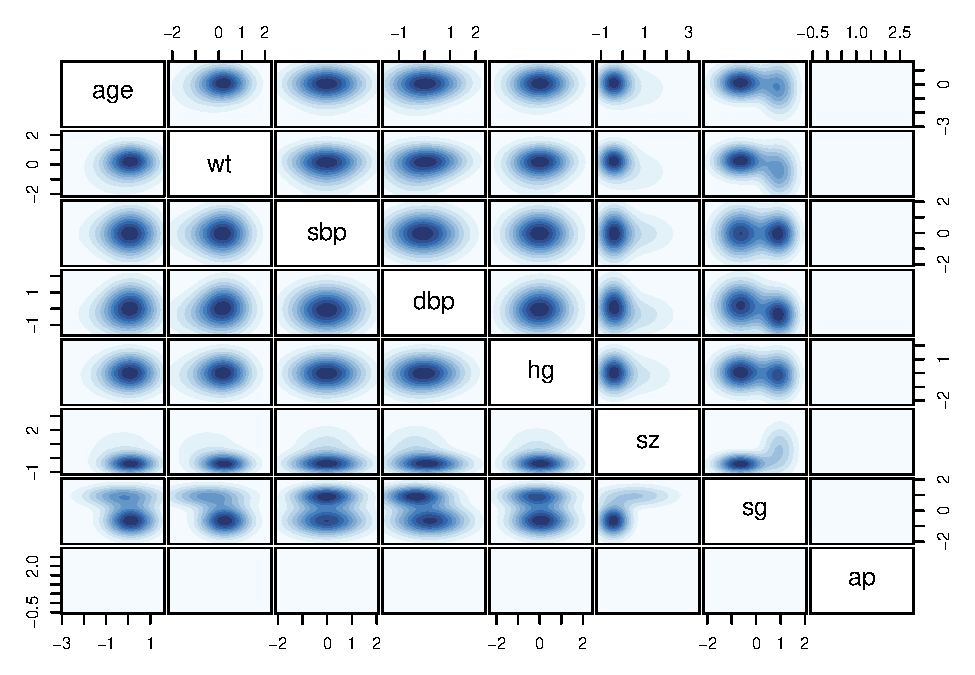
\includegraphics{clustering_files/figure-latex/unnamed-chunk-84-1.pdf}
In this plot, \emph{larger symbols indicate the more uncertain
observations}. The package \emph{factoextra} provides a better
visualization for classification uncertainty on the first factorial
plane (first 2 PCs):

\begin{Shaded}
\begin{Highlighting}[]
\FunctionTok{fviz\_mclust}\NormalTok{(mc, }\StringTok{"uncertainty"}\NormalTok{, }\AttributeTok{palette =} \StringTok{"jco"}\NormalTok{)}
\end{Highlighting}
\end{Shaded}

\begin{verbatim}
## Warning: `guides(<scale> = FALSE)` is deprecated. Please use `guides(<scale> =
## "none")` instead.
\end{verbatim}

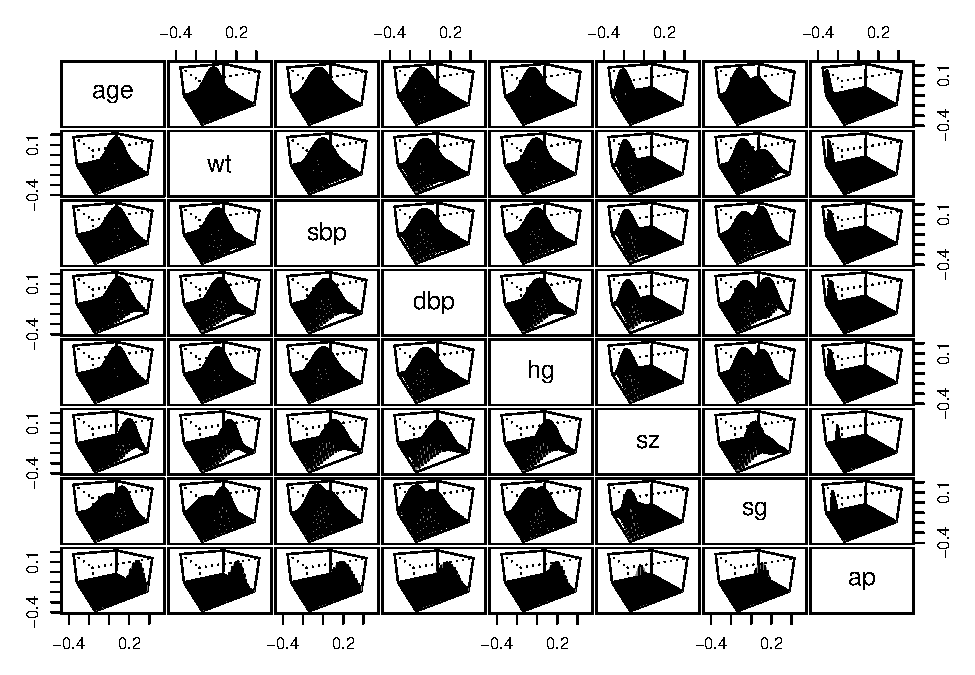
\includegraphics{clustering_files/figure-latex/unnamed-chunk-85-1.pdf}
The plot shows that there are 2 points outside the 2 represented
densities, with one of them (around poisition (2,2)) showed with high
size, indicating a pretty strong uncertainty in its clusters
association.

We can also visaulize a plot of the estimated density:

\begin{Shaded}
\begin{Highlighting}[]
\FunctionTok{plot.Mclust}\NormalTok{(mc, }\AttributeTok{what=}\StringTok{"density"}\NormalTok{, }\AttributeTok{type =} \StringTok{"image"}\NormalTok{, }\AttributeTok{col=}\StringTok{"steelblue"}\NormalTok{, }\AttributeTok{grid =} \DecValTok{200}\NormalTok{)}
\end{Highlighting}
\end{Shaded}

\includegraphics{clustering_files/figure-latex/unnamed-chunk-86-1.pdf}
We can also show 3D graphs of the estimated denisities:

\begin{Shaded}
\begin{Highlighting}[]
\FunctionTok{plot.Mclust}\NormalTok{(mc, }\AttributeTok{what=}\StringTok{"density"}\NormalTok{, }\AttributeTok{type=}\StringTok{"persp"}\NormalTok{)}
\end{Highlighting}
\end{Shaded}

\includegraphics{clustering_files/figure-latex/unnamed-chunk-87-1.pdf}
The density estimation shows the estimated densities by considering eahc
pair of variables: we can see that only some planes show 2 estimated
Gaussians, while the planes of some variables are not able to
discriminate the 2 clusters. For instance, all the plots cosidering
variable `sg' show very clearly the 2 densities.

For instance, to better show the results we discussed above, we may plot
the data using only two variables of interest: we can select `sg' as one
of them (since, as said before, it discriminates very well the 2 groups)
and `dbp':

\begin{Shaded}
\begin{Highlighting}[]
\CommentTok{\# Classification: plot showing the clustering}
\FunctionTok{fviz\_mclust}\NormalTok{(mc, }\StringTok{"classification"}\NormalTok{, }\AttributeTok{geom =} \StringTok{"point"}\NormalTok{, }
            \AttributeTok{pointsize =} \FloatTok{1.5}\NormalTok{, }\AttributeTok{palette =} \StringTok{"jco"}\NormalTok{, }
            \AttributeTok{choose.vars =} \FunctionTok{c}\NormalTok{(}\StringTok{"sg"}\NormalTok{, }\StringTok{"dbp"}\NormalTok{))}
\end{Highlighting}
\end{Shaded}

\includegraphics{clustering_files/figure-latex/unnamed-chunk-88-1.pdf}
As expected, these 2 variables are pretty good in discrimating the 2
groups.

It is possible to use also another dimension reduction method for
visualizing the clustering structure obtained from a finite mixture of
Gaussian densities with the function \emph{MclustDR}.

The estimated directions which span the reduced subspace are defined as
a set of \emph{linear combinations of the original features, ordered by
importance as quantified by the associated eigenvalues}.

\begin{Shaded}
\begin{Highlighting}[]
\NormalTok{drmc }\OtherTok{\textless{}{-}} \FunctionTok{MclustDR}\NormalTok{(mc, }\AttributeTok{lambda =} \DecValTok{1}\NormalTok{)}
\FunctionTok{summary}\NormalTok{(drmc)}
\end{Highlighting}
\end{Shaded}

\begin{verbatim}
## ----------------------------------------------------------------- 
## Dimension reduction for model-based clustering and classification 
## ----------------------------------------------------------------- 
## 
## Mixture model type: Mclust (VVI, 2) 
##         
## Clusters  n
##        1 28
##        2 18
## 
## Estimated basis vectors: 
##          Dir1
## age  0.070479
## wt  -0.196547
## sbp  0.038618
## dbp -0.165069
## hg   0.204623
## sz   0.244341
## sg   0.754339
## ap   0.507014
## 
##                 Dir1
## Eigenvalues   1.2384
## Cum. %      100.0000
\end{verbatim}

In our case, the above method reduced the data to only 1 direction,
which captures most of the clustering structure found with the
model-based algorihm.

The projected plot on this new direction would be:

\begin{Shaded}
\begin{Highlighting}[]
\FunctionTok{plot}\NormalTok{(drmc, }\AttributeTok{what =} \StringTok{"contour"}\NormalTok{)}
\end{Highlighting}
\end{Shaded}

\includegraphics{clustering_files/figure-latex/unnamed-chunk-90-1.pdf}
The plot allows to visualize, with a sort of box-plot, also the
uncertainty in assigning the obsevations into the 2 clusters. The
box-plots show also the values in the new direction (Dir1) of the
observations in each cluster, and we can see that the data are very well
classified into 2 gorups.

We can also visualize the denisity:

\begin{Shaded}
\begin{Highlighting}[]
\FunctionTok{plot}\NormalTok{(drmc, }\AttributeTok{what =} \StringTok{"density"}\NormalTok{)}
\end{Highlighting}
\end{Shaded}

\includegraphics{clustering_files/figure-latex/unnamed-chunk-91-1.pdf}

Save image of all objects created in the session:

\begin{Shaded}
\begin{Highlighting}[]
\FunctionTok{save.image}\NormalTok{(}\AttributeTok{file=}\StringTok{"Clustering.RData"}\NormalTok{)}
\end{Highlighting}
\end{Shaded}


\end{document}
